% ****** Start of file aipsamp.tex ******
%
%   This file is part of the AIP files in the AIP distribution for REVTeX 4.
%   Version 4.1 of REVTeX, October 2009
%
%   Copyright (c) 2009 American Institute of Physics.
%
%   See the AIP README file for restrictions and more information.
%
% TeX'ing this file requires that you have AMS-LaTeX 2.0 installed
% as well as the rest of the prerequisites for REVTeX 4.1
% 
% It also requires running BibTeX. The commands are as follows:
%
%  1)  latex  aipsamp
%  2)  bibtex aipsamp
%  3)  latex  aipsamp
%  4)  latex  aipsamp
%
% Use this file as a source of example code for your aip document.
% Use the file aiptemplate.tex as a template for your document.
\documentclass[%
 aip,
% jmp,
% bmf,
% sd,
% rsi,
 amsmath,amssymb,
%preprint,%
 reprint,%
%author-year,%
%author-numerical,%
% Conference Proceedings
]{revtex4-1}

\usepackage{graphicx}% Include figure files
\usepackage{dcolumn}% Align table columns on decimal point
\usepackage{bm}% bold math
%\usepackage[mathlines]{lineno}% Enable numbering of text and display math
%\linenumbers\relax % Commence numbering lines

\usepackage[utf8]{inputenc}
\usepackage[T1]{fontenc}
\usepackage{mathptmx}
\usepackage{etoolbox}
\usepackage{graphicx}
\usepackage{gensymb}
\usepackage{amsmath}
\usepackage[version=4]{mhchem}
\usepackage{siunitx}
\usepackage{subcaption}
\usepackage[export]{adjustbox}


%% Apr 2021: AIP requests that the corresponding 
%% email to be moved after the affiliations
\makeatletter
\def\@email#1#2{%
 \endgroup
 \patchcmd{\titleblock@produce}
  {\frontmatter@RRAPformat}
  {\frontmatter@RRAPformat{\produce@RRAP{*#1\href{mailto:#2}{#2}}}\frontmatter@RRAPformat}
  {}{}
}%
\makeatother
\begin{document}

\preprint{AIP/123-QED}

\title[Evaluation of Molten Sand, Dust, and Ash Infiltrating Thermal Barrier Coatings: Numerical and Analytical Approaches]{Evaluation of Molten Sand, Dust, and Ash Infiltrating Thermal Barrier Coatings: Numerical and Analytical Approaches}
% Force line breaks with \\
\author{B. Cavainolo}
 \email{brendon.cavainolo@ucf.edu}

 \affiliation{Mechanical and Aerospace Engineering, University of Central Florida}%Lines break automatically or can be forced with \\
\author{R. Naraparaju}%
\affiliation{ 
Institute of Materials Research, German Aerospace Center (DLR)%\\This line break forced with \textbackslash\textbackslash
}%
\author{M-R. Kabir}%
\affiliation{ 
Institute of Materials Research, German Aerospace Center (DLR)%\\This line break forced with \textbackslash\textbackslash
}%

\author{M. P. Kinzel}
 \affiliation{Aerospace Engineering, Embry-Riddle Aeronautical University}%Lines break automatically or can be forced with \\


\date{\today}% It is always \today, today,
             %  but any date may be explicitly specified

\begin{abstract}
Calcium-Magnesium-Alumino-Silicate (CMAS) is a category of atmospheric debris in the form of dirt, sand, and ash that damage thermal barrier coatings (TBC) in aircraft engines. The damage is not a direct result of erosion, but rather, CMAS melts in engines and impacts the TBCs. In this state, the CMAS can infiltrate the TBC microstructure which leads to surface damage from secondary stresses associated with thermal loading and expansion in the micro-structure. Understanding the fluid dynamic processes of the infiltration is key to develop TBCs that mitigate TBC infiltration damage. The fluidic processes are evaluated using micro-structure-resolving, finite-volume, multiphase, volume-of-fluid computational fluid dynamics simulations (CFD). CFD results using experimentally measured temperature-dependent polynomial CMAS viscosity are compared to experiments and analytical models and indicate that feathery-shaped microstructure in TBCs inhibit CMAS infiltration more than rectangular channel TBCs. Such observations are conditional on the Ohnesorge Number (Oh). For low Oh values, the rectangular channel reduces infiltration, while the feathery channel is more effective at reducing infiltration for higher Oh values. 3D CFD results under-predicted experimental and theoretical infiltraiton depth.  
A novel infiltration model for feathery channels, the ``Feathery Pipe-Network Model'' (FPNM) was implemented. FPNM results agree with experiments and other analytical models. Using FPNM in conjunction with the concentric-pipe model achieves a 25\% margin-of-error when evaluated against experimental results. This is a 15\% reduction in error compared to using the open-pipe and concentric-pipe models as the prediction. This enhanced prediction model can lead to safer and more cost-effective aircraft operation in debris-laden environments.



\end{abstract}

\maketitle

\section{\label{sec:intro}Introduction}

Ingestion of Calcium-Magnesium-Alumino-Silicate (CMAS) particles by airplane engines threatens the safety and durability of aircraft. 
%For instance, in 1982, all four engines of a Boeing 747 on British Airways Flight 9 failed when the plane flew through a volcanic ash cloud composed of CMAS. 
When CMAS particles enter the engine, the high temperatures melt the particles that can later be deposited and solidify on engine components \cite{Chen2015}. The deposition of these melted particles can damage the thermal barrier coatings that protect the high-pressure turbine blades and combustor liners, which leads to overheating and damaged surfaces that can cause engine stall \cite{Chen2015}. The issue is not limited to engines on fixed-wing aircraft. Helicopters operating in sandy desert environments are at even higher risk of CMAS damage through engines ingesting sand kicked up during take off and landing\cite{Smialek}. 
%Lastly, these concerns lead to additional financial impacts in terms of lost flights. Such a scenario was demonstrated with the closure of European airspace for six days following the eruption of Eyjafjallajökull in Iceland, which cost commercial airlines an estimated \$1.7 billion \cite{Thehumanconditionblog_2010}. 
It is clear that the relationship of CMAS to aircraft safety and durability is crucial to understand how CMAS behaves inside aircraft engines to prevent damage to both airplanes and the global economy.

Thermal Barrier Coatings (TBCs) are outer ceramic layers applied to aircraft engine components, such as high-pressure turbine blades, to protect them from prolonged exposure to heat \cite{Bennett2005}. These coatings can reduce component temperatures \cite{Sirigiri2018} from around 1700 K to 1200 K. As higher temperature turbines are required for more efficient and higher thrust applications, such coatings are essential for the heat-related aspects of engine design. 
These TBC systems can utilize a variety of materials and be implemented using different methods. One approach uses electron-beam physical vapor deposition (EB-PVD) to manufacture 7\% yttria-stabilized zirconia (7YSZ) coatings. 7YSZ coatings manufactured with this method are favored for their aerodynamic performance and strain compliance benefits over TBCs manufactured with other methods. Note that the top coat is the layer most susceptible to CMAS infiltration \cite{Renteria2007}. 
The columnar microstructure of an EB-PVD coating is shown in Fig. \ref{fig:TBC_scans}, which shows both ``normal'' and ``feathery'' TBCs. These features indicate potential microstructure patterns in TBC coating design. 

\begin{figure}
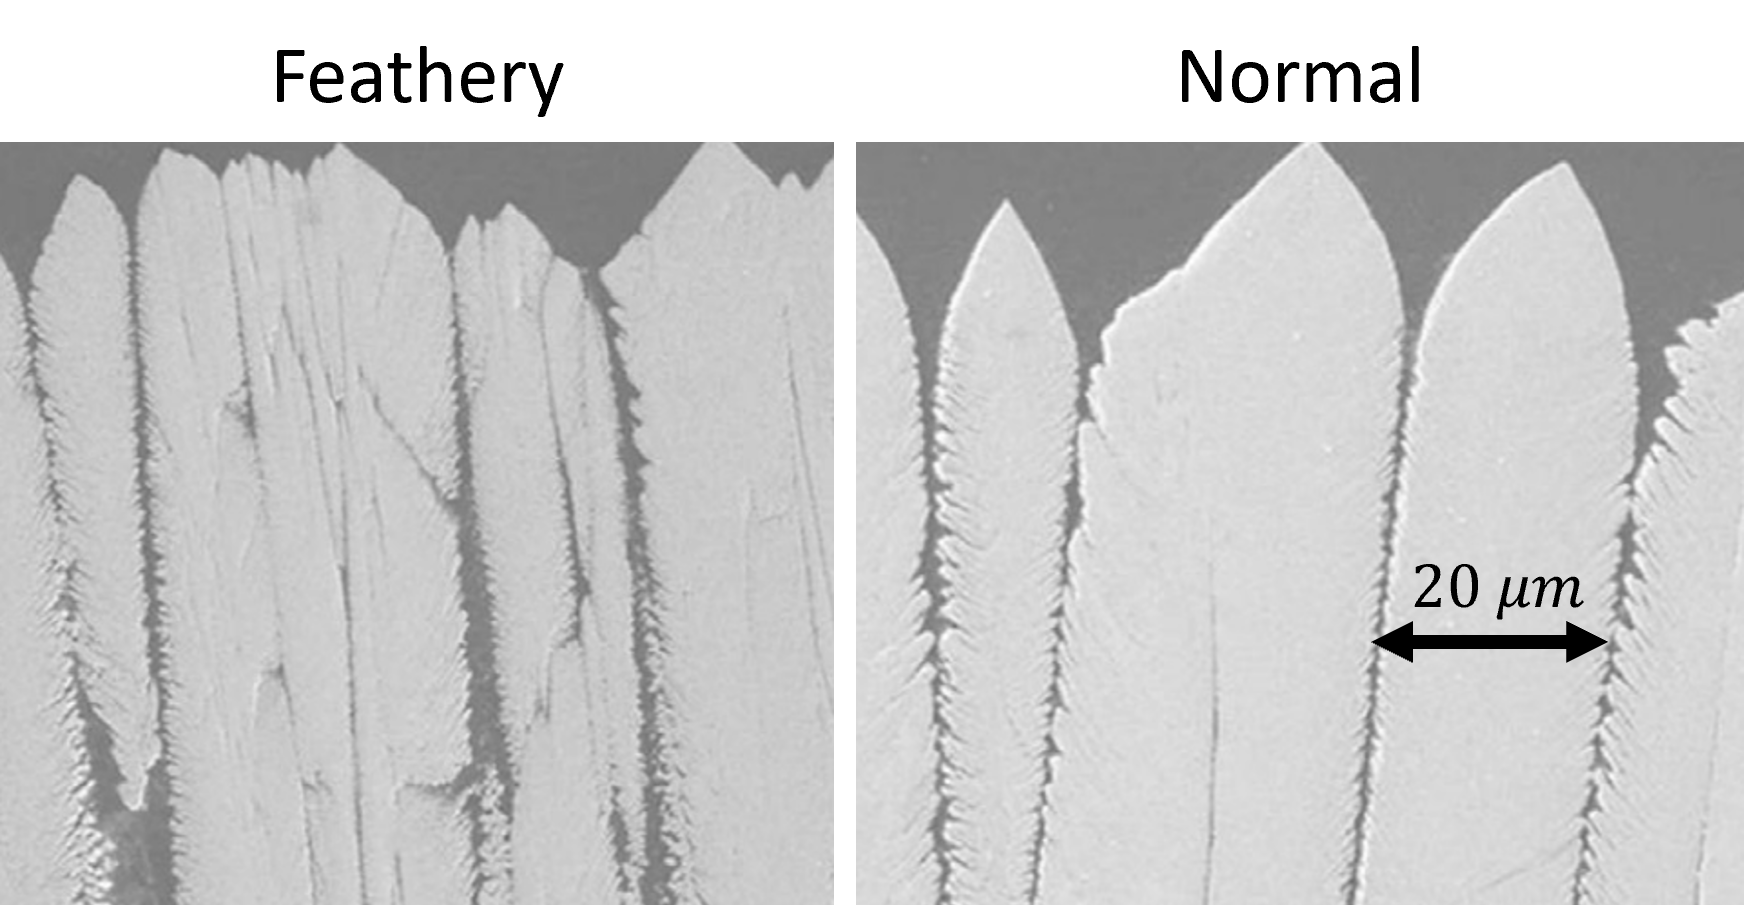
\includegraphics[width=.9\linewidth]{Figures/SEM.png}
\caption{Feathery and parallel microstructure for EB-PVD TBCs under magnification \cite{Naraparaju2017}. These side views were obtained by extracting a cross-section of TBC samples.}
\label{fig:TBC_scans}
\end{figure}

Melted CMAS infiltrates the inter-columnar gaps, and due to the established thermal gradient throughout the coating thickness, some areas of the coating are infiltrated, while others are not. As a result of this, an overall decrease in strain tolerance, and an increase in thermal conductivity is observed, as well as a discrepancy in thermal expansion coefficient between the infiltrated and uninfiltrated regions \cite{KAKUDA2015350,WU20111881, KRAMER200826}. This causes the coating to become susceptible to delamination, if the coating is infiltrated beyond a critical depth \cite{MERCER20051029}. The CMAS attack also causes a sintering phenomena to occur, which also erodes TBCs \cite{Peng2012}. As manufacturers seek to help aero-engines achieve higher temperatures for efficiency gains, molten CMAS is becoming more of a problem \cite{Boyce2012}, because the viscosity of CMAS is temperature dependent \cite{Naraparaju2017}. Thus, higher engine operating temperatures make the CMAS less viscous, and increases its ability to infiltrate the coatings. Depending on composition, most forms of CMAS melt between 1150 - 1250 \degree C \cite{Costa2019,Naraparaju2014,Wellman2010,Kramer2006}.The sintering occurs when the molten CMAS comes into contact with the TBC. In one such case, molten volcanic ash interacted with a YSZ TBC to form yttria-iron garnet \cite{Xia2019}.

%Current literature has explored several important aspects of CMAS interaction with surfaces on aircraft engines. One such study includes a computational model exploring CMAS particle fan-blade interaction \cite{Vogel2018}. This study found the distribution of particle sizes likely to transport past the fan stage in aeroengines \cite{Vogel2018}. Additionally, the effect of CMAS particle size and chemical composition with respect to the time to equilibrate on the nozzle guide vane was explored \cite{Bojdo2019}. The particle’s properties were summarized using the measured thermal Stokes number ($St_{th}=\frac{T_{p,imp}}{T_f}$), which is ratio of particle impact temperature ($T_{p,imp}$) to the air temperature ($T_f$). The study showed that the temperature of particles with a $St_{th}$ below unity equilibrate with the temperature of the surrounding fluid in a fraction of the surrounding fluid’s response time. $St_{th}$ larger than unity led to particles that take much longer than the surrounding fluid’s response time to equilibrate with the surrounding fluid \cite{Bojdo2019}. The correlation provides a useful approach to benchmark new models \cite{Cavainolo2022}. Another numerical model sought to understand how CMAS deposits form on film-cooled turbine vanes \cite{LIU2024131158}.

Previous simulation-based infiltration models have used a finite-element based approach \cite{Kabir, Sirigiri2018}, but this approach comes with several challenges, including difficulties associated with surface tension forces. Kabir and Sirigiri's approach uses a coupled Euler-Lagrange methodology. Here, the TBC is a rigid-body in a Lagrangian domain, and the molten CMAS is a fluid in an Eulerian domain. However, the Eulerian domain is not multiphase (i.e. the air-CMAS interface is not explicitly resolved). Void cells are used instead of an air-phase, and surface tension forces are modeled at the free-surface.

This paper proposes the application of finite-volume method (more specifically and as described in Section~\ref{sec:methods}, the Volume-of-Fluid Method (VOF)) computational fluid dynamics (CFD), to evaluate CMAS infiltration using first principles methods for several idealized TBC geometries. 
Overall, the approach has the potential to push the understanding of infiltration processes. Previous work using this methodology has determined that experimental measurements for viscosity led to more accurate infiltration times. However, there was a large discrepancy between simulated and experimental infiltration times \cite{Cavainolo2023}. 

Many theoretical models exist to evaluate problems that are similar to the CMAS/TBC Infiltration Problem. TBC columns are considered capillary columns \cite{Naraparaju2017}. Thus, seepage-based theoretical models for soil flows may be applicable. One such theoretical model is Layered-Infiltration Theory in which water infiltration depth in soil is estimated based on the properties in the different layers of soil. \cite{ZHAO2024100028}. The open-pipe model (OPM) and concentric-pipe model (CPM) have been derived from soil-based flows, and applied to the CMAS/TBC infiltration problem \cite{CARMAN1997S32, Chapuis2003616, Naraparaju2019}. A theoretical model for predicting capillary imbibition in rocks was developed by correcting the Hagen–Poiseuille equation to account for pore shape and orientation \cite{Benavente2002}. The Lucas-Washburn equation was also modified to model large porous structures instead of isolated columnar channels \cite{Cai2021}. There is no shortage of theoretical models that could help solve the CMAS/TBC problem. However, all of these models would need to be expanded and specifically tuned to accommodate CMAS/TBC infiltration. The OPm and CPM sought to accomplish this, but results fell within a wide margin of error compared to experiments \cite{Naraparaju2019}. OPM and CPM assume a large porous medium, and the microstructure boils down to a couple of geometric parameters. So, a new thoertical model is needed to accurately capture effects complicated microstructures, such as the ''feathery`` microstructure in Fig. \ref{fig:TBC_scans}. So, additionally, this work proposes the ``Feathery Pipe-network Model'' (FPNM) as a way to describe the flow in an isolated feathery TBC columnar gap. 
%However, the validity for these theoretical models to describe the CMAS/TBC infiltration in a single isolated column is not fully understood. The pipe models are intended to describe the bulk flow of fluid through a porous medium \cite{Naraparaju2017}, whereas capillary flow models describe the flow in an isolated TBC columnar gap. This brings forth a basic question, \textit{how accurate are theoretical porous media models for analyzing isolated TBC columns with complex shapes?}



In summary, this work seeks to do the following: 1) Provide details of a methodology in which CMAS infiltration into a TBC is directly resolved using numerical simulation 2) Compare the directly-resolved simulation results to expected results from the analytical pipe models \cite{Naraparaju2019} (Shown in Appendix \ref{sec:app:RaviPipeModels}), the FPNM, and previous experiments measured at the German Aerospace Center (DLR) \cite{Naraparaju2019}. 3) Characterize the infiltration process based on physical and geometric properties.

\section{Methods}
\label{sec:methods}

\subsection{Computational Fluid Dynamics Simulations}
The simulation methodology used in our efforts\cite{Cavainolo2023, Cavainolo2022} is based on the finite-volume-based, VOF CFD approach. These models are built into Star-CCM+ \cite{starccm}, and are not unique or novel. Hence, the numerical methods will only be described briefly, and the reader is referred to the Star-CCM+ User Manual for more information on the specifics \cite{starccm}. However, the implementation of these methods is novel in that VOF has not yet been used to analyze the CMAS infiltration problem. Lattice-Boltzmann methods are commonly used to resolve complicated geometries \cite{Zhang2011}. However, it has been shown that Navier-Stokes based methods are capable of resolving microfluidic problems as well \cite{LeHenaff2022}.

The first step in simulating the infiltration of CMAS was to ensure the VOF method is a valid approach for capturing the melting-solidification of a CMAS particle. A mesh independence study was conducted in previous work \cite{Cavainolo2022}, and it is shown that melting particles between the solidus and liquidus temperatures of CMAS can be accurately resolved with the VOF method. For multiphase physics, the Eulerian Multiphase Volume-of-Fluid method was used to simulate the interactions between the two Eulerian phases, air, and CMAS.  Modeling surface tension properly is critical as the infiltration is driven by capillary forces. The governing equations of the VOF-CFD model from  Star-CCM+ \cite{starccm} include conservation equations for mass,

\begin{equation}
\label{consMass:equation}
    \frac{\partial}{\partial t}\int_{V}\rho dV+\ \oint_{A}{v\cdot d\Vec{A}}=\ \int_{V}\left(S\right)dV\ ,\ S=\ \sum_{i}{S_{\alpha_i}\rho_i},
\end{equation}

\noindent momentum,

\begin{eqnarray}
\label{consMomentum:equation}
    &&\frac{\partial}{\partial t}\int_{V}\rho vdV+\oint_{A}{\rho v\times v}\cdot\ dA \nonumber\\
    &&=\oint_{A}{\rho I\cdot d\ A}+\oint_{A}{T\cdot d\ A}+\int_{V}\rho gdV\ \\
    &&+\int_{V}{f_bdV}-\sum_{i}\int_{A}{a_i\rho_iv_{d,i}\times v_{d,i}dA}\nonumber
\end{eqnarray}


\noindent and energy,

\begin{eqnarray}
\label{consEnergy:equation}
   &&\frac{\partial}{\partial t}\int_{V}\rho EdV+\oint_{A}\left[\rho Hv+p+\alpha_i\rho_i{H_iv}_{d,i}\right]\cdot dA=\nonumber \\
   &&=-\oint_{A}{{\dot{q}}^{\prime\prime}\cdot d A} \\
   &&+\oint_{A}{T\cdot v d A}+\int_{V}{S_EdV}+\ \int_{V}{f_bdV}.\nonumber
\end{eqnarray}


\noindent Equations \ref{consMass:equation}-\ref{consEnergy:equation} couple to the Eulerian Multiphase VOF approach, which solves a transport equation for volume fraction of a phase $i$ ($\alpha_{i} = V_{i}/V$) and is formulated as follows 

\begin{eqnarray}
\label{VOFtrans:equation}
    &&\frac{\partial}{\partial t}\int_{V}\alpha_{i}dV+ \oint_{A}\alpha_{i}v\cdot dA\nonumber\\
    &&=\int_{V}\left(S_{\alpha_{i}}-\frac{\alpha_i}{\rho_i}\frac{D\rho_{i}}{Dt}\right)dV\\
    &&-\int_{V} \frac{1}{\rho_{i}}\nabla\cdot \left(\alpha_{i}\rho_{i}v_{d,i}\right)dV\nonumber
\end{eqnarray}

\noindent In these equations, the subscript $i$ denotes a particular phase (in this case, air or CMAS), and $S_{\alpha_{i}}$ is a source term that controls phase change. This equation is discretized using High-Resolution Interface Capturing (HRIC). HRIC blends the upwind and downwind solution around an interface to satisfy a Courant number limit (i.e. Co = 1.0), and if the Courant number is exceeded, then the HRIC scheme reverts back to a standard upwind scheme, which results in a smeared interface. This smeared interface can be corrected by implementing temporal subcycling. The general idea of temporal subcycling is shown in Eq. \ref{eq:GeneralTempSubCycle}, where the right-hand side of the equation is a single source term that combines the right-hand side contributions from Eq. \ref{VOFtrans:equation}. The use of a multiphase model is a key departure from Kabir and Sirigiri's work \cite{Kabir, Sirigiri2018} because it allows for direct resolution of the capillary effects at the air-CMAS interface, as opposed to a modeled free-surface boundary driven downward with a prescribed capillary pressure.

\begin{eqnarray}
\label{eq:GeneralTempSubCycle}
    &&\alpha^{n+\Delta t}V - \alpha^{n}V + \int_{t^{n}}^{t^{n+\Delta t}}( \ \sum_{A}\alpha_{f}(s) v \cdot da)\nonumber\\
    &&=\int_{t^{n}}^{t^{n+\Delta t}}(S(\alpha (s),...)ds
\end{eqnarray}


\noindent In this work, an implicit multi-stepping version of this temporal subcycling is employed, which gives an unconditionally stable solution, and a sharp interface is achieved if $\frac{CFL}{N_{imp}} \leqslant 0.5 $. The sub-iterations calculated with Eq. \ref{eq:implicitMultiStep1} are summed to get the overall contribution for the whole time step.

\begin{eqnarray}
\label{eq:implicitMultiStep1}
    &&\alpha_{i+1}V - \alpha_{i}V + \tau( \ \sum_{A}\alpha_{f,i+1}(\tau) v \cdot da) \nonumber \\
    &&=\tau(S(\alpha^{n+\Delta t},...) ~ for~ i = 1, 2, ..., N
\end{eqnarray}

A drawback of using the VOF method for the infiltration is the very small time steps required to resolve the CMAS infiltration. So, adaptive time-stepping combined with sub-iterations was used to balance computational speed and accuracy. A free-surface condition was enforced so that the Courant number ($Co = \frac{u \Delta t}{\Delta x}$) at the interface was around 1.0. Such a criterion is demanded to accurately capture interfacial dynamics. 
%The VOF method requires the use of a segregated solver (i.e. the energy equation is solved in a separate system of equations). This solver is second-order accurate in space, and first-order accurate in time. However, the lower-order time accuracy is offset by the implicit multi-stepping in the segregated VOF solver, described in Equations \ref{eq:GeneralTempSubCycle} - \ref{eq:implicitMultiStep1}. 
These equations are solved using a segregated SIMPLE-C, solver using numerics that are second-order accurate in space, and first-order accurate in time. Note that the lower-order time accuracy is offset by the implicit multi-stepping in the segregated VOF solver, described in Equations \ref{eq:GeneralTempSubCycle} - \ref{eq:implicitMultiStep1}. 

\subsubsection{Solidification Model}
\label{sec:solidmodel}
Solidification is captured in the CMAS using an approach that couples to the VOF method. Within the CMAS VOF phase, there is a solid-coloring function, $\alpha_s^*$, given as   
%in the following way in Star-CCM+'s implementation of the VOF method \cite{starccm}

\begin{equation}
    \alpha^{*}_{s} = \begin{cases}
    1 & T^{*} < 0 \\
    f(T^{*})& 0<T^{*}<1 \\
    0& 1 < T^{*}
    \end{cases},
    \label{eq:solidificationModel}
\end{equation}

\noindent where
\begin{equation}
    T^{*} = \frac{T - T_{solidus}}{T_{liquidus} - T_{solidus}}.
\end{equation}

\noindent In this effort, the latent heat of fusion, $h_{fusion}$, is important to consider and is captured through 

\begin{equation}
    h_{is}^{*} = h_{is} + \left( 1 - \alpha_{s}^{*}\right)h_{fusion}
    \label{eq:latentHeat}
\end{equation}

%\subsection{Flow-stop submodel}
\noindent Such a model ensures that energy associated with phase-change effects are accounted for. Beyond this, a ``flow-stop submodel'' is employed to stop the fluid flow in the cells that have reached a particular solid threshold (the flowability threshold, $FT$). Specifically, when the solid volume fraction from Equations \ref{eq:solidificationModel} - \ref{eq:latentHeat} reaches the $FT$, the velocity in that cell is set to zero. In order to maintain numerical stability in the solution of the continuity equation, the density in the stopped cells must be held constant, which is achieved with the flow-stop mass compensation option. For the numerical studies in this work, the flow-stop submodel was turned off, except for the solidification characterization in Section \ref{sec:solidificationCharacterization}, where it was varied. 

\subsubsection{Geometry, Mesh, and Boundary Conditions}

In this study, several different microstructures (shown in Fig.~\ref{fig:dimensions}) are evaluated to represent the micro-scale pores. Firstly, a rectangular micro-channel, represented by a 2D plane extending infinitely into the z-direction. The rectangular channel's purpose is to serve as a benchmark; a case that allows the numerical methods in this model to be compared to analytical models for capillary flow. 

This rectangular geometry was  evaluated against the results from a feathery micro-channel. This feathery micro-channel was scanned by DLR scientists \cite{Sirigiri2018} and a representation of the geometry was converted into a 2D and 3D geometry, shown in Fig. \ref{fig:dimensions}. The 3D geometry is just the 2D geometry extended into the page. Here, the feathery pattern shown on the right is repeated downward until the TBC column is 200 $\mu m$ deep. This is half the depth of the TBC sample used in experiments \cite{Naraparaju2019}. It should be noted that a typical TBC coating on an aircraft component is $\approx 150 - 180~\mu m$ deep. The TBC coating used in the experiments was larger in order to perform longer kinetic experiments. 

The geometry is then meshed using an unstructured trimmed-cell mesh which can be seen in Fig. \ref{fig:mesh}. The 3D simulations used adaptive mesh-refinement (AMR) at the air-CMAS interface. 

Due to limitations in the 2D model, a separate set of boundary conditions had to be used in the 2D and 3D models. The 2D model is not capable of spontaneously producing capillary flow, unlike the 3D model. The interface resolution, paired with the lack of a inflow/outflow boundary in the z-direction causes the inertial forces to dominate the flow in the 2D model. So, the flow in the 2D model must be ''jump-started`` by an enforced pressure gradient. The boundary conditions for the 2D model are summarized in Table \ref{tab:2DboundaryConditions}. 

Boundary conditions and domain dimensions for the 3D model are summarized in Fig. \ref{fig:dimensions}b and Table \ref{tab:3DboundaryConditions}. Note that only the feathery geometry was simulated in 3D. All flow boundary conditions are zero-gradient, that is, pressure and volume fraction on each of the boundaries is the same as the fluid entering/leaving the boundary. These boundary conditions are important because they ensure the flow of the CMAS is purely driven by capillary effects and not pressure gradients. While it could potentially make more sense to use engine operating pressures for the simulation's reference pressure, this domain was set up to be more in line with experiments conducted by Naraparaju et al. \cite{Naraparaju2014, Naraparaju2017, Naraparaju2019} to ensure the comparison to experimental data is as accurate as possible.

For both the 2D and 3D geometries, conjugate heat transfer was considered by setting the TBC as a solid region, the walls of the TBC were prescribed as a temperature gradient, (i.e. $\Delta T_{x}$), of -1 $K/\mu m$, such that the top of the coating is close to a typical operating temperature for an engine environment. The gradient is defined this way to relate the simulation to the TBC sample that was used in experiments \cite{Naraparaju2019}, which was around 400 $\mu m$ deep, and manages to be around 400 K cooler at the bottom of the TBC than the top, such that the operating temperature is below the melting point of the materials used. It should be noted there is only a gradient in the x-direction, so any walls on the same x-plane will have a constant temperature, and any walls along the same y-plane will have a temperature that varies. 

The wall contact angle of the CMAS phase is expected to be somewhere between 40 and 70 degrees based on experiments \cite{Naraparaju2019}. 
These values are temperature dependent though. For simplicity, a constant wall contact angle of 67 degrees was used \cite{Naraparaju2019}.

The thermal gradient described above for the boundary conditions was also used as the initial temperature condition for both the fluid region and solid region. The fluid domain's initial velocity was set such that there was a very small downward velocity. This is done because it helps with convergence in the first calculations in the simulation.  An additional assumption made in the CFD is that TBC walls are perfectly smooth, which is not necessarily the case in an actual TBC.  Gravity was also enabled to capture any infiltration effects from buoyancy. Turning on gravity also adds the Boussinesq Approximation to the energy equation to account for natural convection. However, the effects of natural convection do not dominate the flow. 


\begin{figure*}
    \centering
    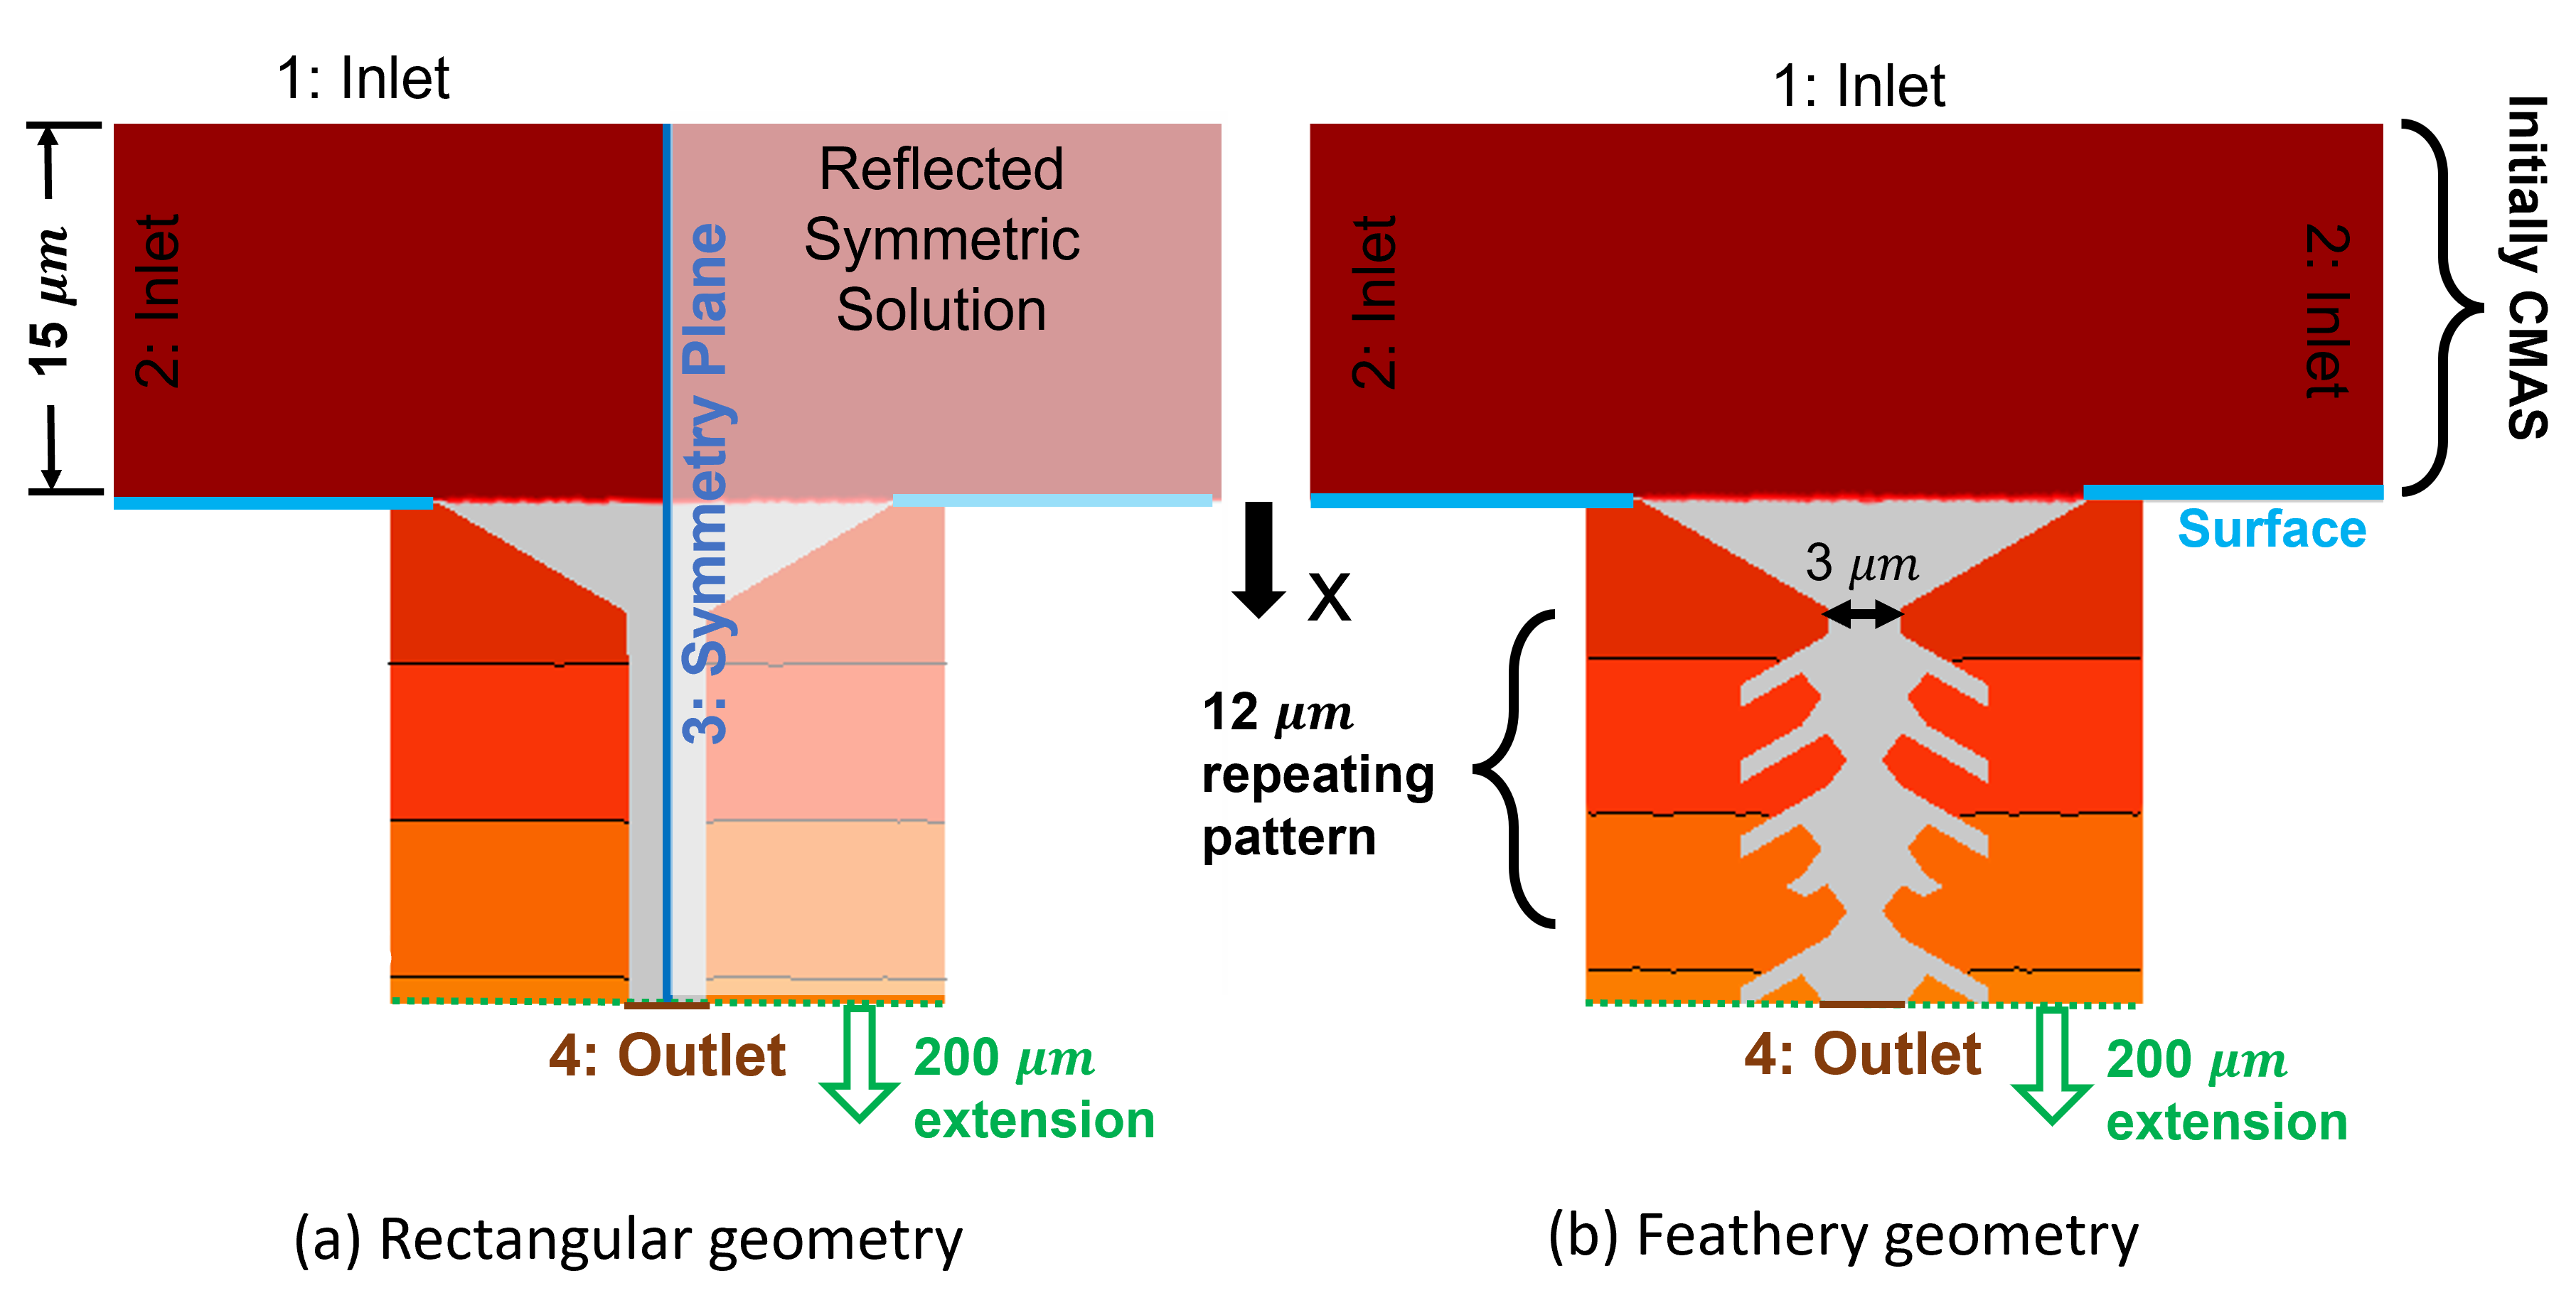
\includegraphics[width=0.9\linewidth]{Figures/dimensionsTwoView.png}
    \caption{Dimensions and boundary conditions applied to two channel types. The contours indicate the thermal boundary conditions in the solid. The dark-red colored area is filled with CMAS which infiltrates into the gray region (air). The red-to-orange gradient represents the decreasing temperature within the TBC as depth increases.}
%    \caption{rectangular (left) and feathery (right) geometries with labeled dimensions and boundary conditions. The dark red colored area shows the starting position of CMAS, and the gray area shows the starting position of air. The red-to-orange gradient represents the decreasing temperature in the TBC as the depth increases.}
    \label{fig:dimensions}
\end{figure*}

% \begin{figure*}
%     \centering
%     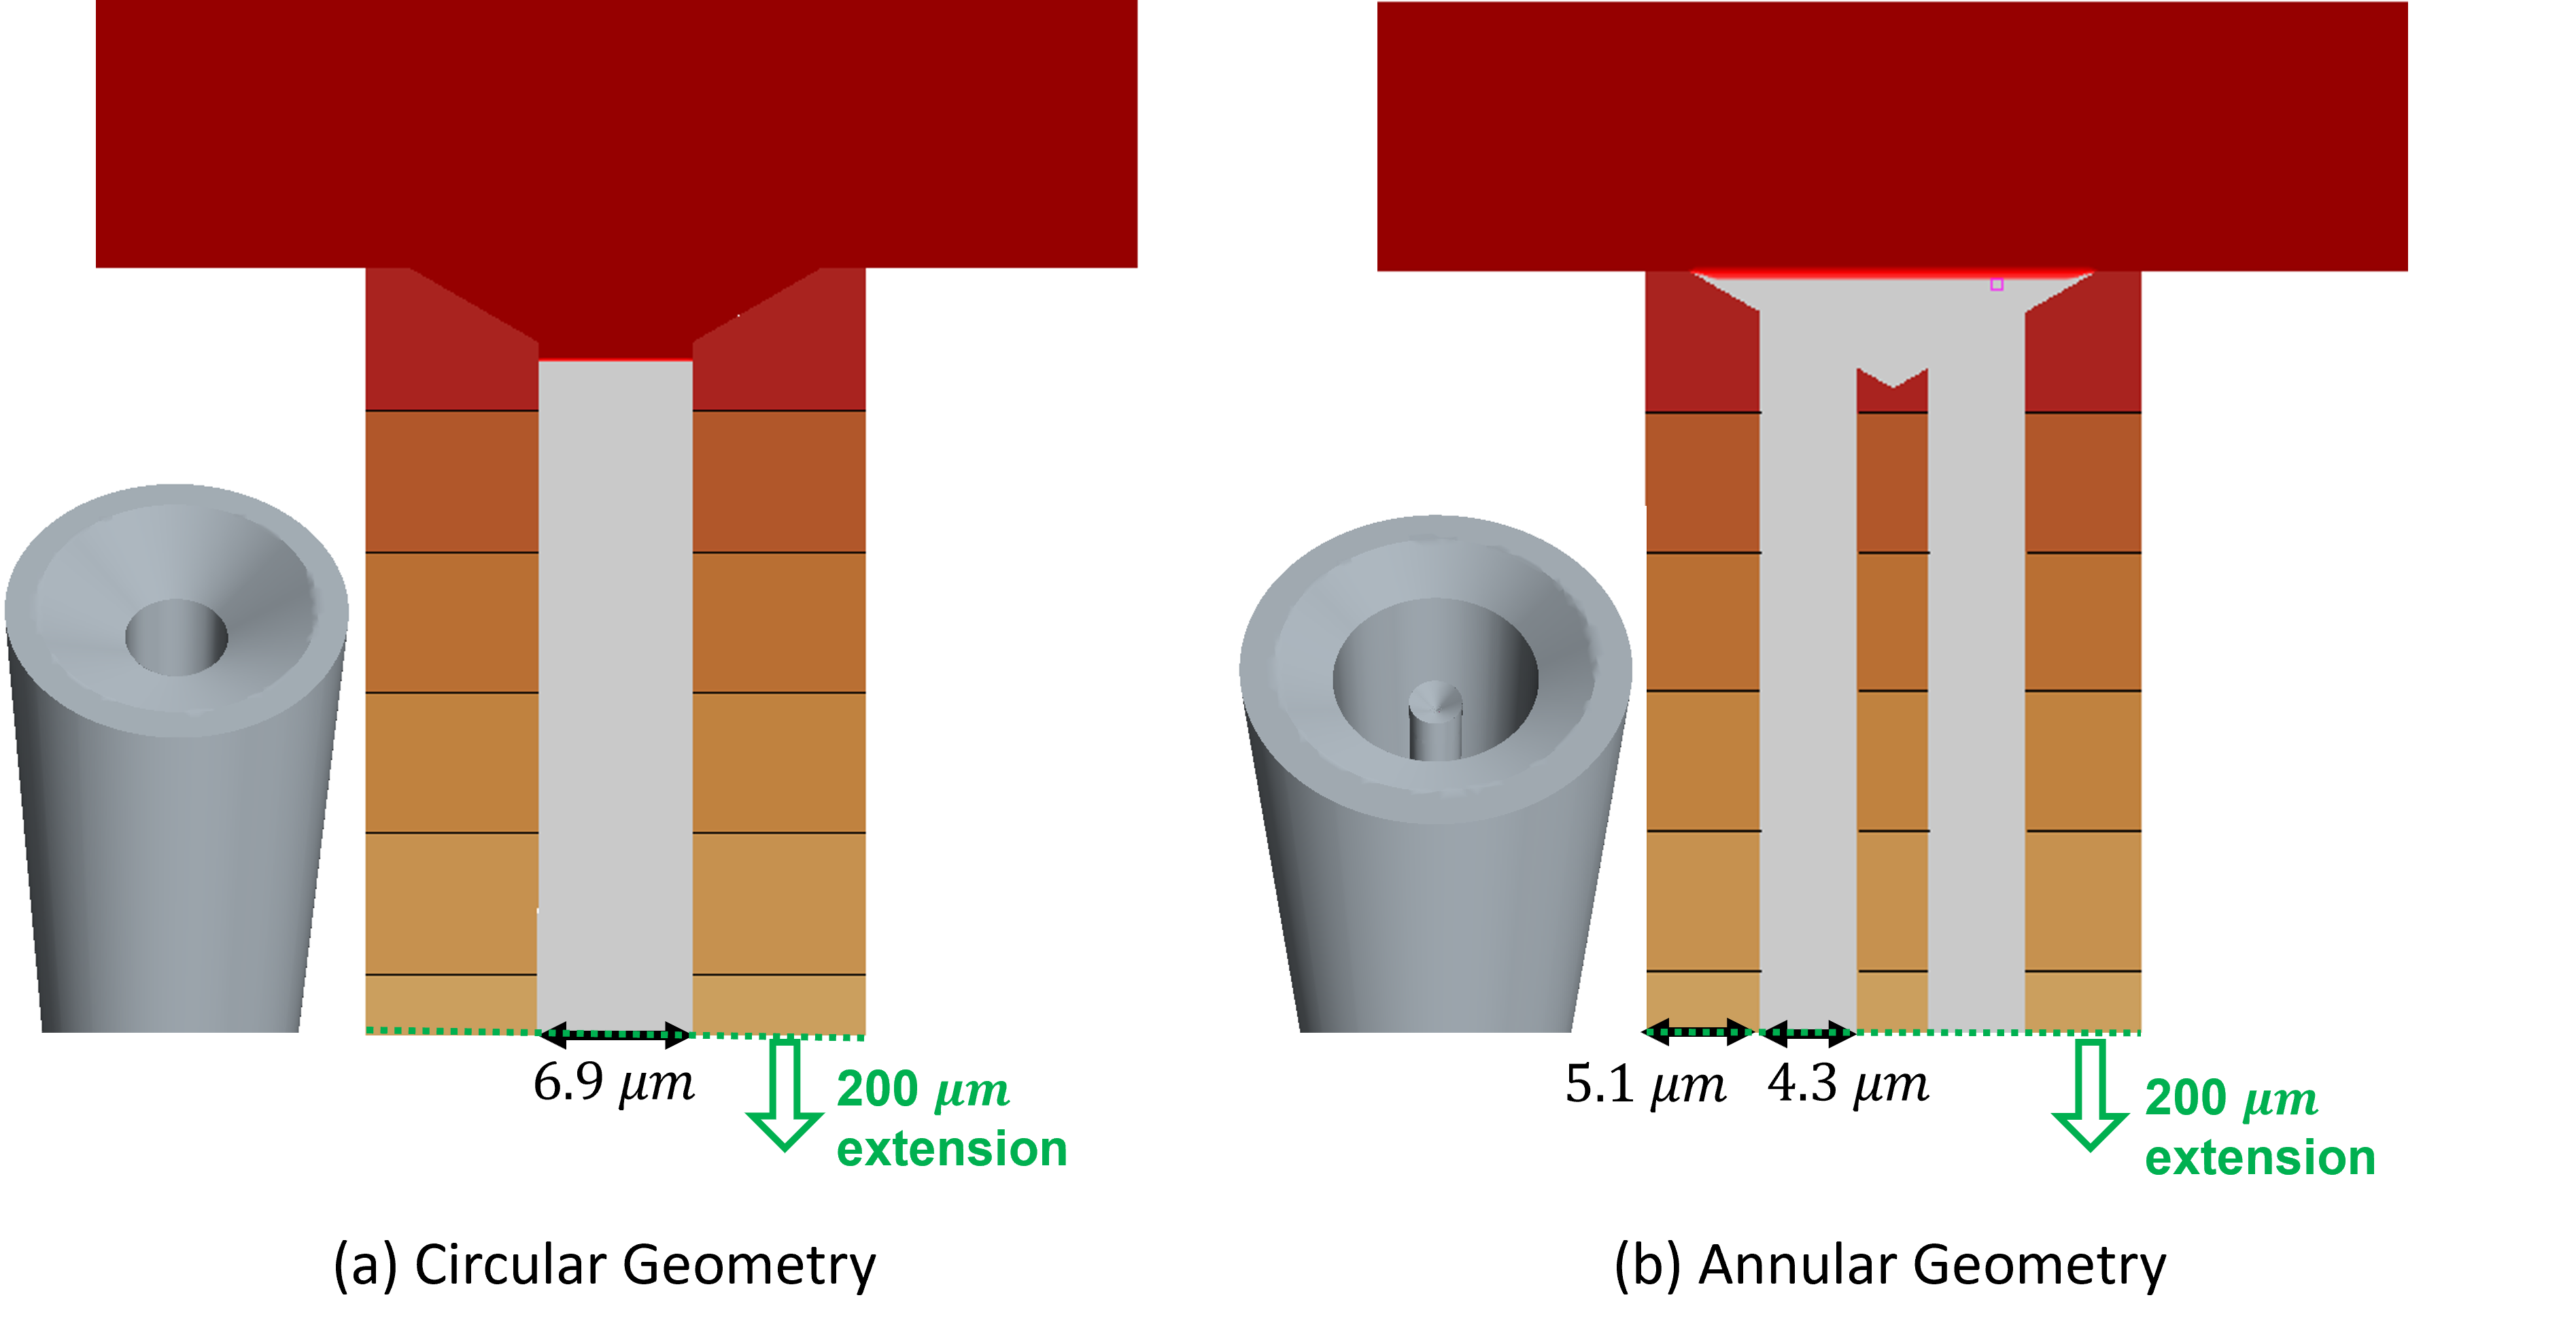
\includegraphics[width=0.9\linewidth]{Figures/3d_geometries.png}
%     \caption{Axisymmetric geometries and dimensions (labeled). Boundary conditions are similar to discussed in Fig.~\ref{fig:dimensions}}
%     \label{fig:3D_Geometries}
% \end{figure*}

\begin{figure}[htp!]
\centering
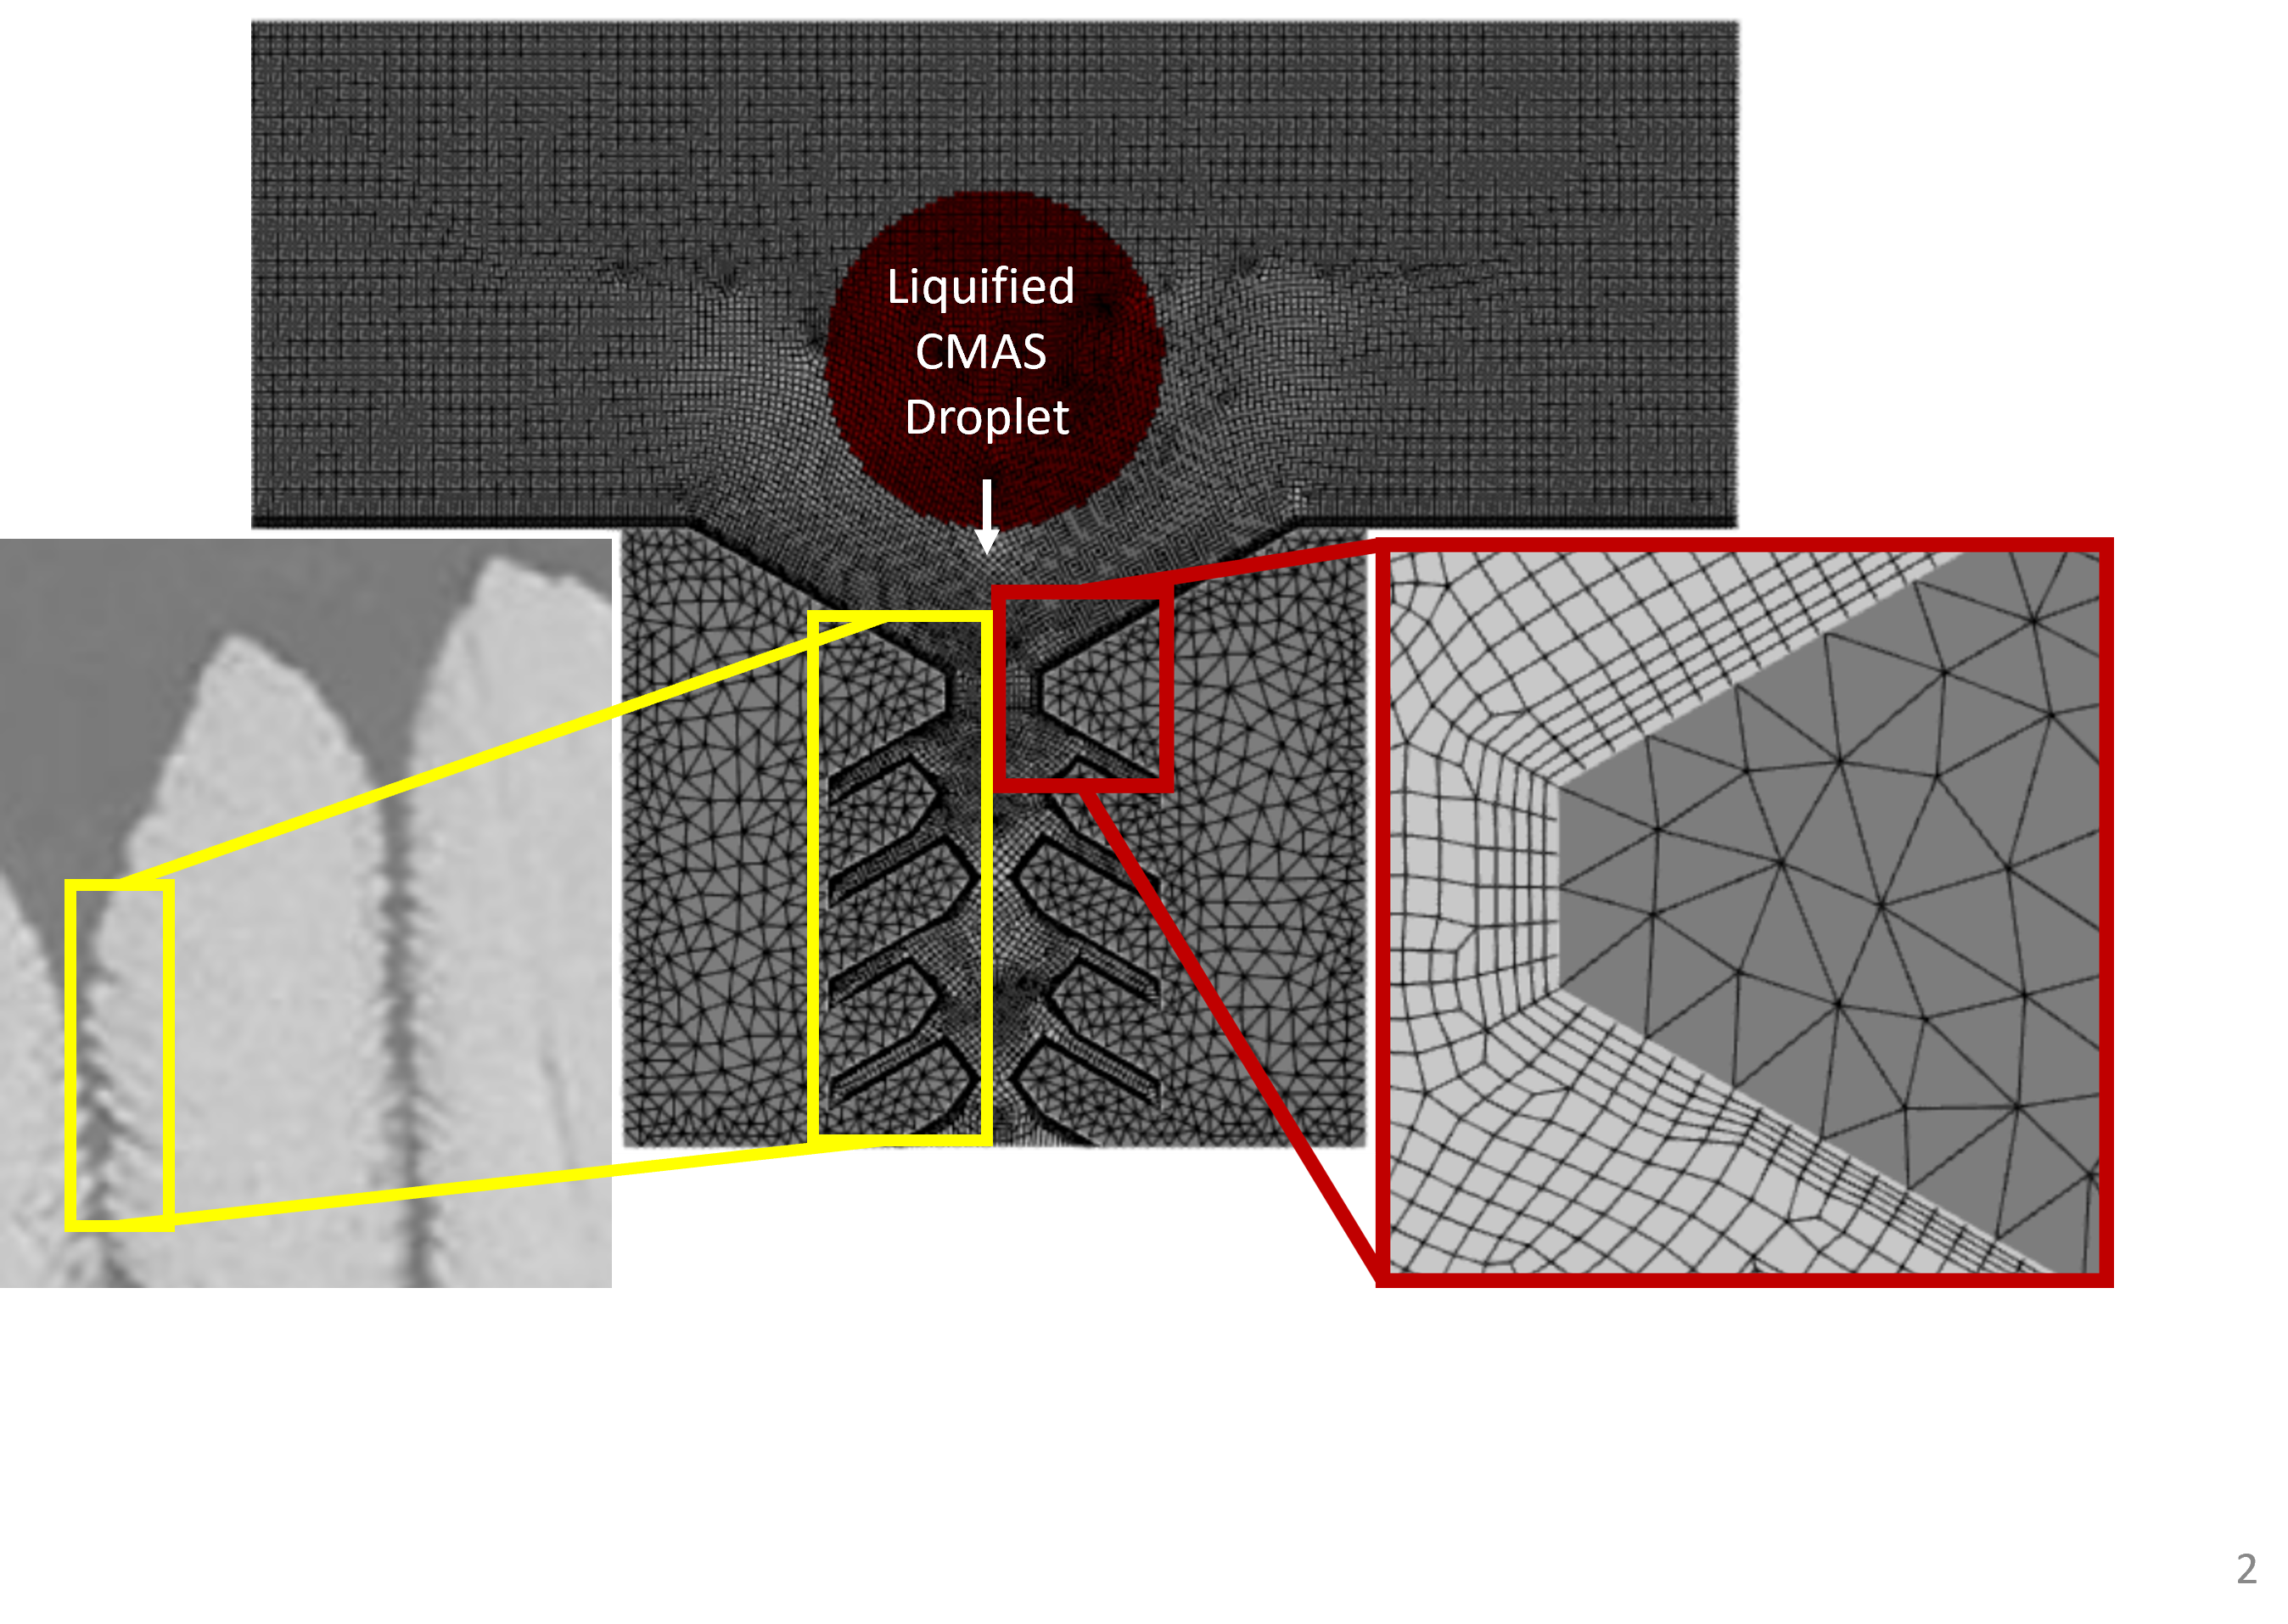
\includegraphics[width=\linewidth]{Figures/mesh_and_sem_compare.png}
\caption{Overall computational mesh and domain compared to a scanning electron microscope (SEM) image (yellow). The mesh has zoomed-in view in the near-wall region. Also, the feather shape can be correlated to feathers from the SEM image.}
\label{fig:mesh}
\end{figure}



\begin{table}[htp!]
\caption{\label{tab:2DboundaryConditions} Summary of labeled boundary conditions for the 2D domain (pressure values with respect to reference pressure $P_{ref} = 101325$ Pa)}
\centering
\begin{ruledtabular}
\begin{tabular}{cccc}
Label &Type& Boundary Condition& Value (Units)\\\hline
1& Inlet&Pressure & 3.0 $MPa$\\
-& -&Temperature& $1530$ K\\
2& Inlet&Pressure& 3.0  $MPa$\\
-& -&$T(x)$& 1530 -$\Delta T_{x}\times x$ (x in $\mu m$)\\
3& Symmetry&- & -\\
4& Outlet&Pressure& -50 $MPa$\\
-& -&Temperature & $1324$ K \\
5& Walls&$T(x)$& 1530 -$\Delta T_{x}\times x$ (x in $\mu m$)\\
\end{tabular}
\end{ruledtabular}
\end{table}

\begin{table}[htp!]
\caption{\label{tab:3DboundaryConditions} Summary of labeled boundary conditions for the 3D domain (pressure values with respect to reference pressure $P_{ref} = 101325$ Pa). Note that the 3D domain is the same as the 2D domain shown in \ref{fig:dimensions}b, but extended in the -Z and +Z directions (into and out of the page). The -Z and +Z boundary conditions are unlaballed, but are shown in this table.}
\centering
\begin{ruledtabular}
\begin{tabular}{cccc}
Label &Type& Boundary Condition& Value (Units)\\\hline
1& Inflow/Outflow & $\frac{\partial P}{\partial x}$ & 0\\
-& -&Temperature& $1530$ K\\
2& Inflow/Outflow& $\frac{\partial P}{\partial x}$ & 0\\
-& -&$T(x)$& 1530 -$\Delta T_{x}\times x$ (x in $\mu m$)\\
3& Symmetry&- & -\\
4& Inflow/Outflow& $\frac{\partial P}{\partial x}$ & 0\\
-& -&Temperature & $1324$ K \\
5& Walls&$T(x)$& 1530 -$\Delta T_{x}\times x$ (x in $\mu m$)\\
-Z and +Z & Inflow/Outflow& $\frac{\partial P}{\partial x}$ & 0\\

\end{tabular}
\end{ruledtabular}
\end{table}

%\subsection{Air Phase and Porosity}
Additionally, due to the 2D model assumptions and incompressible air phase, air pockets within the feather gaps demanded paths to escape. To accomplish this, %the interface between the fluid and solid regions 
the fluid-solid interface
was modeled as %set as 
a porous boundary to allow the air to escape. The boundary was modeled with a pressure rise calculated as
\begin{equation}
\label{porous:equation}
    \Delta P = -\rho (\alpha |v_n| + \beta)v_n.
\end{equation}
%The rate at which air was allowed to escape with 
Here, the values of the external pressure ($\Delta P$), inertial resistance ($\alpha$), and viscous resistance ($\beta$), were set to the ambient pressure (i.e., $0 Pa$), 100 (dimensionless), and $1 \frac{m}{s}$, respectively. With this model, the air can escape the pore based on the local pressure and is limited to a maximum velocity of $0.01 \frac{m}{s}$ according to Eq. \ref{porous:equation}.



% \subsection{Modifications to the Governing Equation for Capillary Flow in a rectangular micro-channel}

% For analytical benchmarking, this works seeks to modify an existing governing equations for capillary flow in a micro-channel. One such governing equation for capillary flow in a rectangular micro-channel is given as \cite{Waghmare2012}

% \begin{equation}
%     \left( h^* + C_{1} \right) \frac{d^{2}h*}{dt^{*2}} + C_{2} \left( \frac{dh^{*}}{dt^{*}} \right)^{2}  + \left(C_{3} + C_{4}h^{*} \right) \frac{dh^{*}}{dt^{*}} + C_{5}h^{*} + C_{6} = 0.
%     \label{eq:ODEeq}
% \end{equation}

% \noindent Note that $t^{*}$ and $h^{*}$ are non-dimensional time and depth, and are respectively normalized by $t_{0} =\frac{ \rho 4B^{2} }{12\mu} $ and $ h_{0} = 2B $. The modified coefficients are given and described in Table \ref{tab:ODECoeff}.

% \begingroup
% \setlength{\tabcolsep}{10pt} % Default value: 6pt
% \renewcommand{\arraystretch}{2} % Default value: 1
% \begin{table}[htp!]
% \caption{\label{tab:ODECoeff} Description of Constants and Coefficients in Equation \ref{eq:ODEeq}}
% \centering
% \begin{tabular}{lcccccc}
% \hline
% Coefficient & Definition&\\\hline
% $C_{1}$ & $\frac{0.55}{\alpha_{1}} \sqrt{\gamma}$ \\
% $C_{2}$ & $\frac{\alpha_{1}}{1.158 + \alpha_{1}}$  \\
% $C_{3}$ & $\frac{1}{3\alpha_{1}\left[ \Phi^{4} -6exp\left( \frac{-\Phi^{2}t^{*6}}{3}\right)\right] \times \left[ \Phi^{6} \left( 1-\alpha_{1} \right) - 4\Phi^{2}exp\left( \frac{-\Phi^{2}t^{*6}}{3} + 3\Phi^{4}  \right) \right]}$  \\
% $C_{4}$ &  $\frac{0.295 \sqrt{\gamma}}{\alpha_{1}}$     \\
% $C_{5}$ &  $\frac{Bo}{144\alpha_{1} Oh^{2}}$    \\
% $C_{6}$ &  $\frac{\gamma - cos\theta}{72\alpha_{1} Oh^{2}}$\\
% $\alpha_{1}$ & $\frac{\left[ \Phi^{4} - 4exp\left(- \frac{\Phi^{2}t^{*}}{3}\right) \right]}{\left[ \Phi^{4} - 6exp\left(- \frac{\Phi^{2}t^{*}}{3}\right) \right]}$\\
% $\Phi$ & $\lambda_{n}B$ \\
% $\lambda_{n}$ &$\frac{\left( 2n-1\right)\pi}{2B}$ \\
% \hline
% \end{tabular}
% \end{table}
% \endgroup

% The ODE is solved numerically by converting it from a second-order ODE into a system of first-order ODEs, seen in Equation \ref{eq:linearSystem}. This system is stiff, so it is solved numerically using Matlab's ODE23s algorithm.

% \begin{equation}
% \label{eq:linearSystem}
% \begin{bmatrix}
%     y^{'}_{1} \\
%     y^{'}_{2}
% \end{bmatrix} = 
% \begin{bmatrix}
%     y_{2} \\ 
%     \frac{-C_{2} y_{2}^{2} - (C_{3} + C_{4} y_{1}) y_{2} - C_{5} y_{1} - C_{6}}{y_{1} + C_{1}}
% \end{bmatrix}
% \end{equation}

% Initial conditions from simulations are used to construct a solution to this equation. This solution is compared to simulated, analytical, and experimental results.

\subsection{Theoretical Model: FPNM}
\label{sec:pipeNetworkMethod}
This works also seeks a more representative, but still intuitive way of describing the flow within the feathery microstructure of a TBC. Therefore, a feathery-pipe-network model (FPNM)  is formulated and proposed and is based on considering a network of capillary channels. This model was inspired by a capillary flow electrical circuit analogy \cite{Mikaelian2020}. However, the circuit analogy does not allow for configurations matching the TBC gap. So, FPNM is proposed. Theoretical model development has also shown that the Lucas-Washburn equation can indeed be extended into larger, heterogeneous porous media \cite{Cai2021}, but this theoretical model is also more generalized and is difficult to specifically model the configurations seen in Figures \ref{fig:TBC_scans} and \ref{fig:dimensions}.
In FPNM, there is a primary channel, with other secondary channels extending (almost) perpendicular from the primary tube. In the context of the FPNM, these secondary channels, effectively retard the primary-channel flow. The FPNM model formulation demands added input using the following variables (which can be referenced in Fig. \ref{fig:FPNM_cartoon}:

\begin{itemize}
    \item $n$, the number of secondary channels affecting the flow in the primary channel (increases as depth of CMAS in primary tube increases)
    \item $h_{p}$, the depth of the CMAS in the primary channel
    \item $h_{s}$, the depth of the CMAS in a secondary channel
    \item $B$ is the inter-columnar gap (width of the primary channel)
    \item $b$ is the feather gap width
    \item $\Delta b$ is the separation between each feather gap
    \item $\theta$ is the feather angle
    \item $L_{s}$ and $L_{p}$ are the lengths of the primary channel (the coating depth), and the feather length respectively
\end{itemize}

\begin{figure}
    \centering
    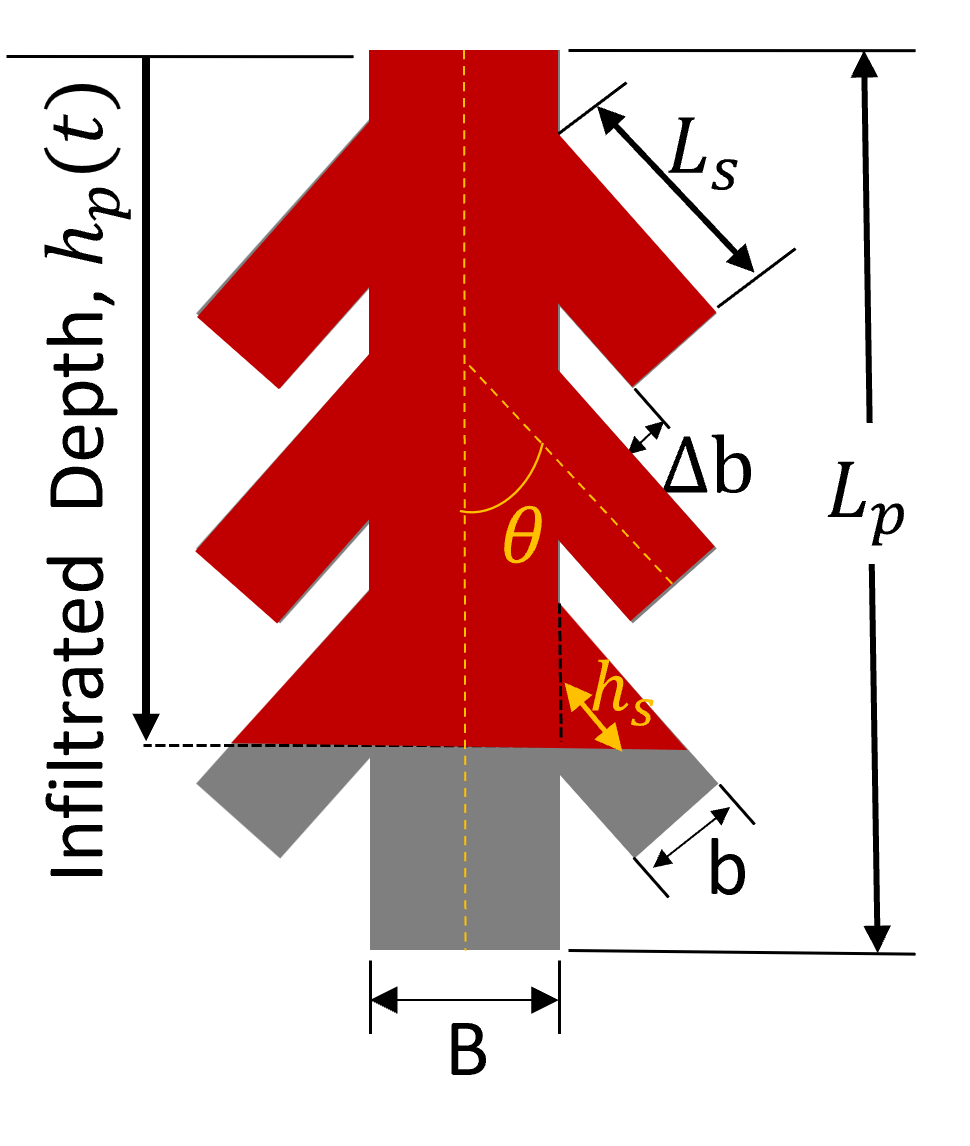
\includegraphics[width=\linewidth]{Figures/FPNM_cartoon.png}
    \caption{Visual representation of geometric parameters describing FPNM}
    \label{fig:FPNM_cartoon}
\end{figure}

\noindent A visual representation of these variables is shown in Fig.~\ref{fig:FPNM_cartoon}. It is proposed to adapt these variables into the Washburn model\cite{Washburn19213}, which is given as

\begin{equation}
    \frac{dh}{dt} = \frac{d^{2}}{\mu}\frac{\Delta P}{L}.
\end{equation}

\noindent Where $\Delta P = \sigma/d$, this is the proposed relation for the primary channel, as so

\begin{equation}
    \frac{dh_{p}}{dt} = \frac{B^{2}}{\mu}\frac{\Delta P}{L_{p}}.
\end{equation}

\noindent However, an additional term to account for the flow in the secondary channels must be added (i.e. the flow that is causing ``resistance'' in the primary channel). If we assume that this resistance, $R_{s}$, takes the form

\begin{equation}
    R_{s} = \frac{b^{2}}{\mu}\frac{\Delta P}{L_{s}}cos\theta,
\end{equation}

\noindent it can be said that 
\begin{equation}
        \frac{dh_{p}}{dt} = \frac{B^{2}}{\mu}\frac{\Delta P}{L_{p}} -ncos\theta\frac{b^{2}}{\mu}\frac{\Delta P}{L_{s}}.
\end{equation}

\noindent The number of feathers affecting the flow in the primary channel ($n$) increases as the depth of CMAS in the primary channel increases. However, $n$ can be solved directly since the primary channel height ($h_p$), feather width ($b$), and feather gap width ($\Delta b$) are known.

\begin{equation}
    n = 2\frac{h_{p}}{b + \Delta b}.
\end{equation}

\noindent So the overall equation becomes, after substituting $\Delta P = \sigma/d$,

\begin{equation}
    \frac{dh_{p}}{dt} = \frac{B \sigma}{h_{p}\mu} - 2 cos\theta\left(\frac{h_{p}}{b + \Delta b} \right)\frac{b \sigma}{L_{s}\mu}.
\end{equation}


\noindent Now, it is assumed that the time it takes for the flow to infiltrate the feathers, $L_{s}(t)$ is much smaller than the time scale of the primary flow. So, $L_{s}(t)$ can be integrated with respect to time to get 
\begin{equation}
    L_{s}\left( t \right) = \sqrt{\frac{\sigma t b}{\mu}}.
\end{equation}

\noindent Implementing this definition and rearranging yields a time-dependent differential equation

\begin{equation}
    \frac{dh_{p}}{dt} = \frac{\sigma B}{\mu} \frac{1}{h_{p}(t)} - 2 cos\theta h_{p}(t) \left( \frac{1}{b+\Delta b} \right) \sqrt{\frac{\sigma b}{\mu t}}
    \label{eq:FPNM_dimensional}
\end{equation}

\noindent which can be rearranged and rewritten in terms of the $Oh$ with respect to the primary channel, as well as non-dimensional variables $h_p^* = h_p/B$, and $t^* = t/t_{B}$, where $t_{B} = \sqrt{\frac{\rho B^{3}}{\sigma}}$
\begin{eqnarray}
\label{eq:FPNM_non-dimensional}
    &&h_{p}^{*}\left(t^{*}\right)\frac{dh_{p}^{*}}{dt^{*}} + 2 cos\theta \sqrt{\frac{\rho B^{3}}{\sigma}} \left( \frac{1}{b+\Delta b} \right)\left(h_{p}^{*}\left(t^{*}\right)\right)^{2} \\
    && + \sqrt{\frac{\sigma b}{\mu B^{2}}} \frac{1}{\sqrt{t^{*}}} h_{p}^{*} \left(t^{*}\right) = Oh_{B}^{-1}. \nonumber
\end{eqnarray}
% \begin{equation}

% \end{equation}


\noindent Here, we have a nonlinear, first-order ODE that is readily solvable. To account for non-linear variations of fluid properties, such as viscosity, Eq.~\ref{eq:FPNM_non-dimensional} is solved in small time increments, and the properties are updated after each increment. Importantly, the maximum viscosity is limited to the viscosity the CMAS achieves at its solidification temperature. Viscosity does not change above this point in FPNM.

%\subsection{Properties of the TBC and CMAS}
\subsection{TBC and CMAS Material Properties}
\label{subsec:CMAS/TBCProp}
The material properties of both the CMAS and the TBC affect infiltration. Some of these properties are widely documented, such as thermal conductivity of the TBC \cite{Han2023}. Table \ref{tab:CMAS and TBC properties} shows the properties used for both the CMAS and the TBC. Blank entries are properties not relevant to the model (in this case, for the solid TBC region). Importantly, silicate melts tend to obey Hooke's Law and behave like a viscoelastic material \cite{Sharon1997}.Thus, CMAS is considered an incompressible, Newtonian fluid \cite{Naraparaju2017,Naraparaju2019, Sharon1997}.  While an equation-of-state has been implemented for CMAS in previous numerical efforts \cite{Sirigiri2018}, the density variation was found to be incredibly small. Thus, constant density is assumed. 
Another key departure from Kabir and Sirigiri's work \cite{Kabir, Sirigiri2018} is the implementation of temperature-dependent properties in both the CMAS and TBC, as seen in Table~\ref{tab:CMAS and TBC properties}. Particularly, the temperature-dependent viscosity of CMAS would greatly affect the flow kinetics because of the thermal gradient imposed at the outer boundary of the TBC. Capillary flow in microchannels is greatly dependent on viscosity \cite{Washburn19213}, so the rheological properties of CMAS, particularly viscosity, will affect the flow solution. At lower temperatures, the viscosity will be higher, and thus the infiltration will be slower. Higher temperatures lead to less viscous CMAS and faster infiltration. To account for this, the viscosity is modeled as a polynomial from experimental measurements \cite{Naraparaju2019} and is implemented as a nonlinear solution step in the CFD solver.

\begin{table}[htp!]
\caption{\label{tab:CMAS and TBC properties} Summary of thermal and physical properties of CMAS and TBC}
\centering
\begin{ruledtabular}
\begin{tabular}{lcccccc}
Property & CMAS& TBC\\\hline
Thermal Conductivity (W/m-K)& 1.15 \cite{Bakal2017} & tabular \cite{Han2023} \\
Specific Heat (J/kg-K)& 900 \cite{KAKUDA2015350} & tabular \cite{Han2023} \\
Density (kg/m$^3$)& 2690 \cite{BANSAL20153901}& 4800 \cite{KAKUDA20092583}\\
Dynamic Viscosity (Pa-s)& Polynomial \cite{Naraparaju2019}& -\\
Latent Heat of Fusion (MJ/kg)& $19.73$ \cite{Costa2019}& -\\
Surface Tension (N/m)& 0.4 \cite{Bravo2020}& -\\
Solidus Temperature (K) & 1503\cite{Naraparaju2014} &-\\
Liquidus Temperature (K) & 1523\cite{Naraparaju2014} &-\\
\end{tabular}
\end{ruledtabular}
\end{table}



\section{Results and Discussion}
Here, the results from the simulations and analytical models are discussed, starting with a mesh sensitivity study, moving on to comparing the analytical models with the numerical results, and finally characterization based on several properties is considered.

\subsection{CFD Model}
\subsubsection{Benchmark: Capillary Rise in a Circular Tube}

Since CMAS infiltration in a TBC is a capillary-dominated flow, the methodology above must be validated for use with such flows.
A canonical configuration for a capillary-driven flow is the transient capillary rise in a circular tube.
This case is typically used when validating multiphase numerical methods \cite{GRUNDING2020142, Shiri2022}. 
To do this, a 3D cylindrical tube was set up using the same methods described in Section \ref{sec:methods}.
Constant viscosity water with no solidification model was used in place of the molten CMAS, and the domain was isothermal.
The tube's dimensions and boundary conditions are shown in Fig.\ref{fig:benchmark_diagram}. Zero pressure gradient boundaries were used to ensure only capillary forces are driving the flow. Only water was allowed to enter the tube, while water and air can exit the tube.

\begin{figure*}
    \centering
    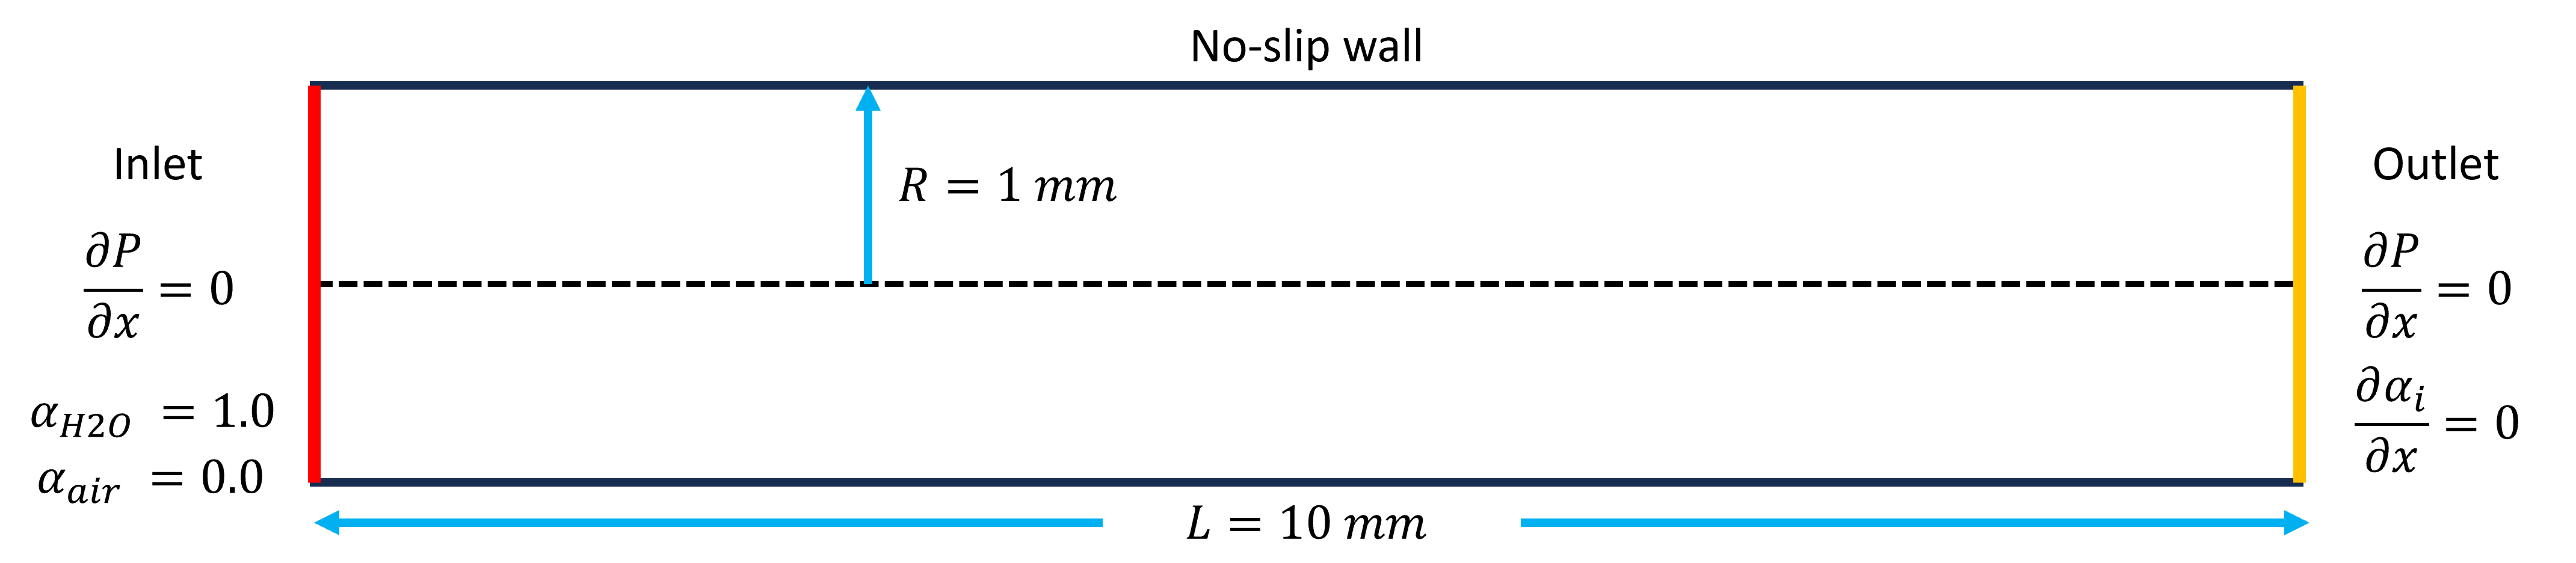
\includegraphics[width=\linewidth]{Figures/capillaryRiseDiagram.png}
    \caption{Diagram showing the dimensions and boundary conditions for the benchmark capillary rise in a tube case.}
    \label{fig:benchmark_diagram}
\end{figure*}

Fig. \ref{fig:capillaryRise} shows the volume fraction of water throughout the capillary rise simulation. Here, a meniscus spontaneously forms due to the capillary action at the tube wall. Then, the meniscus continues to ascend. The ascent rate of the meniscus according to an analytical formulation of the Lucas-Washburn equation \cite{HAMRAOUI2002415} should be around 0.32 $m/s$  (Note that this value was achieved ignoring effects of dynamic contact angle, as this phenomenon is ignored in the present study). The ascent rate of the meniscus in this benchmark CFD model is around 0.36 $m/s$. A 12.5\% error is achieved between the analytical Lucas-Washburn equation and the CFD model. The qualitative observations in Fig. \ref{fig:capillaryRise} and the quantitative comparison between the analytical Lucas-Washburn equation and the CFD model demonstrate the ability of the simulation methodology to resolve capillary-driven flow. 

\begin{figure}
    \centering
    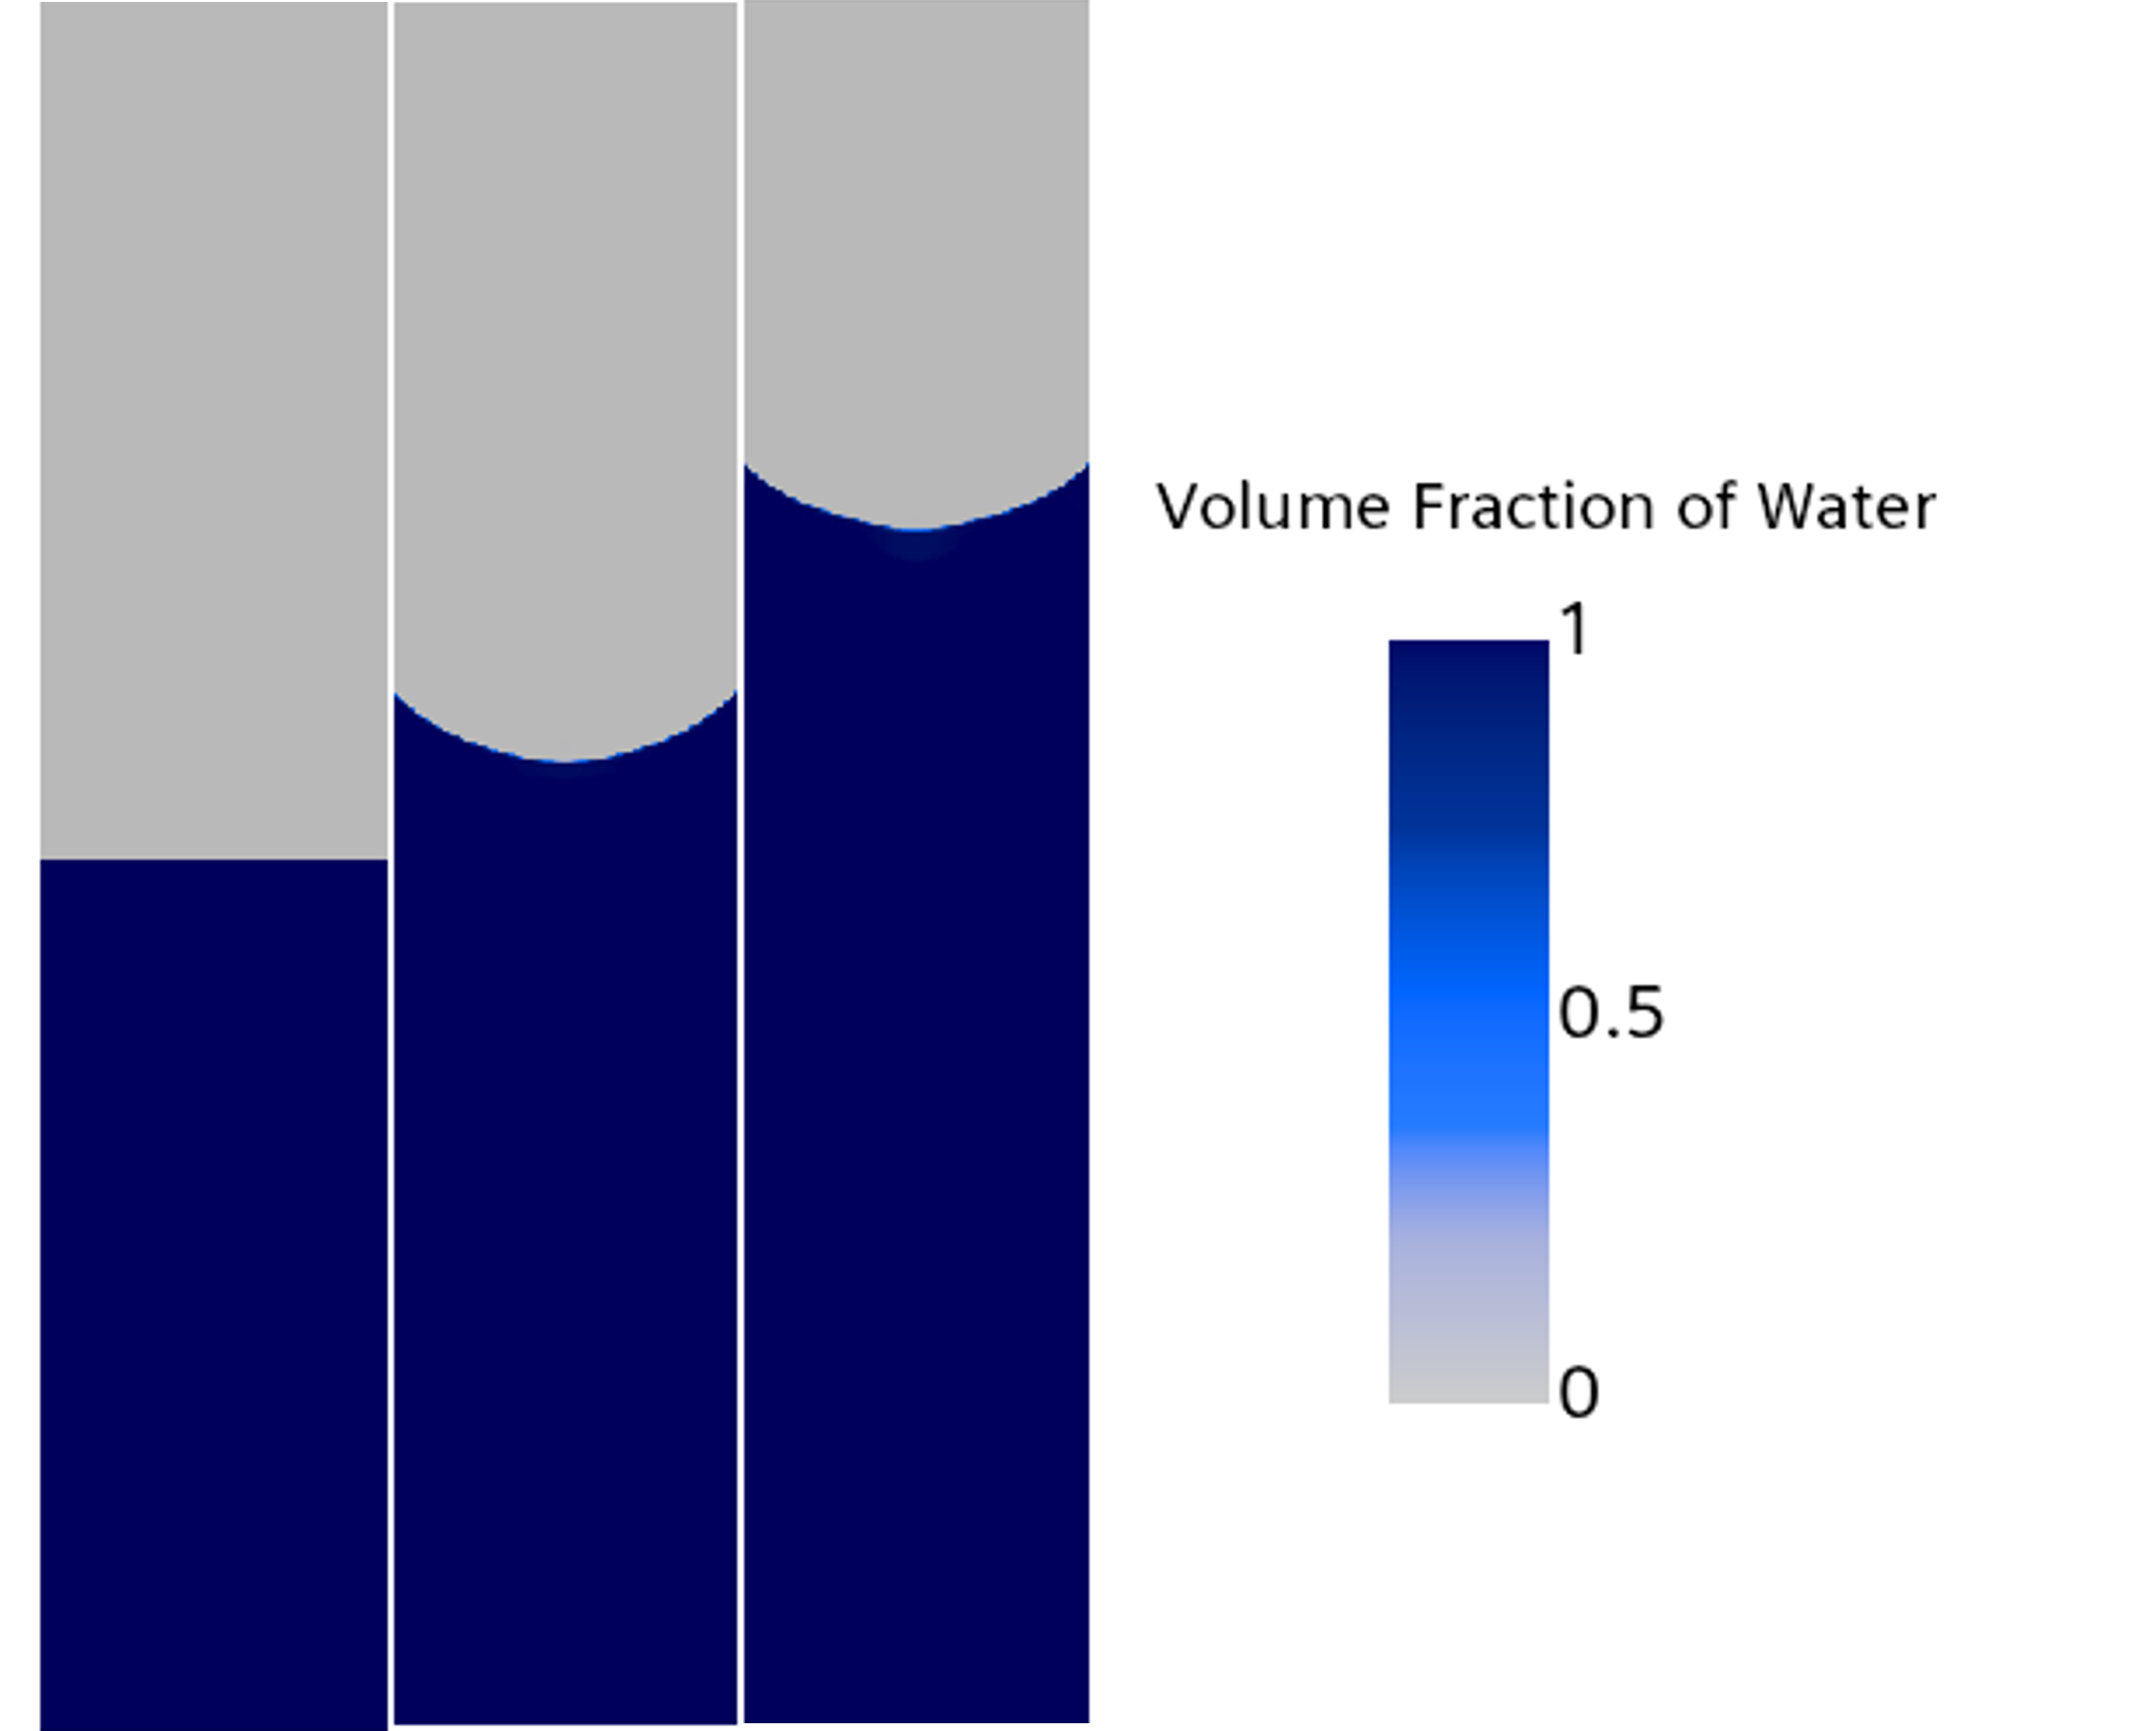
\includegraphics[width=\linewidth]{Figures/validation_capillaryRise.png}
    \caption{Simulated capillary flow in a tube at three different stages. From left to right, the flow is initialized halfway up the tube and there is no meniscus. Next, the meniscus spontaneously forms and begins to move upward. Last, the meniscus has moved much further up the tube than where it started. This shows that capillary rise is resolved.}
    \label{fig:capillaryRise}
\end{figure}

\subsubsection{Validation: Mesh Sensitivity Study}
A mesh sensitivity study was conducted where a single CMAS droplet was resolved. The droplet's initial velocity was 0.2 $m/s$, allowing for quick impingement of the TBC. From there, the droplet infiltrates via capillary action as normal. The setup for this is shown in Fig. \ref{fig:mesh}. The infiltration depth at 0.1 s of physical time was extracted for several levels of refinement. The results in Fig. \ref{fig:meshSensResults} and Table \ref{tab:meshSensResults} show convergence. Since results vary incredibly little with finer mesh sizes, a mesh with a base size of ${1.4\times 10^{-7}}$ m will be used for further simulations. Performing the formal grid convergence index (GCI) calculations \cite{ECA2014104, celik2008procedure} shows that the results in Table \ref{tab:meshSensResults} imply oscillatory convergence, because  $0<\epsilon_{21}/\epsilon_{32}=\ 0.004<1$, and a GCI of $7.5\times 10^{-4}$.
%The physical time to extract the infiltration depth was chosen because beyond that time, error accumulates in the low-fidelity simulation, where the mass of CMAS grows beyond the initial value, causing the result to be non-physical. This non-physical phenomenon can be seen in the coarsest mesh in Fig. \ref{fig:mesh-a}, and the result becomes more clear in Fig. \ref{fig:mesh-b} - \ref{fig:mesh-d}. 

% \begin{figure}[htp!]
%     \begin{subfigure}{0.5\linewidth}
%         \centering
%         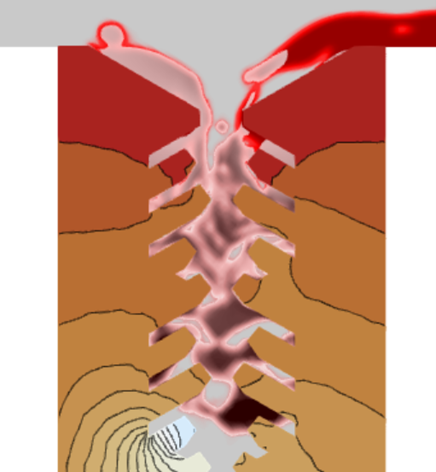
\includegraphics[scale=0.75]{Figures/coarsestMesh.png}
%         \caption{$2.1x10^{-7}$}
%         \label{fig:mesh-a}
%     \end{subfigure}
%     \begin{subfigure}{0.5\linewidth}
%         \centering
%         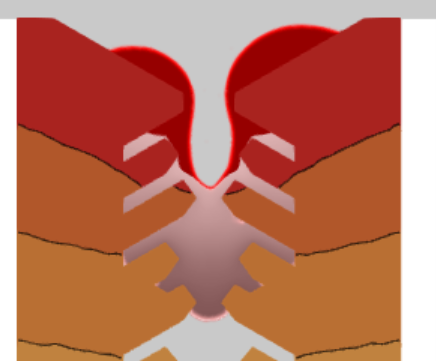
\includegraphics[scale=0.75]{Figures/fineMesh.png}
%         \caption{$1.4x10^{-7}$}
%         \label{fig:mesh-b}
%     \end{subfigure}
%     \begin{subfigure}{0.5\linewidth}
%         \centering
%         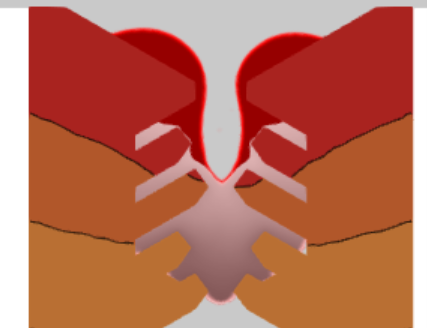
\includegraphics[scale=0.75]{Figures/finerMesh.png}
%         \caption{$1.0x10^{-7}$}
%         \label{fig:mesh-c}
%     \end{subfigure}
%     \begin{subfigure}{0.5\linewidth}
%         \centering
%         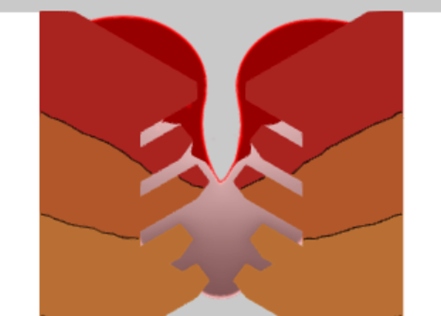
\includegraphics[scale=0.75]{Figures/finestMesh.png}
%         \caption{$7.5x10^{-8}$}
%         \label{fig:mesh-d}
%     \end{subfigure}
%     \caption{CMAS Infiltration at different levels of mesh refinement}
%     \label{fig:mesh-refine}
% \end{figure}

\begin{figure}
    \centering
    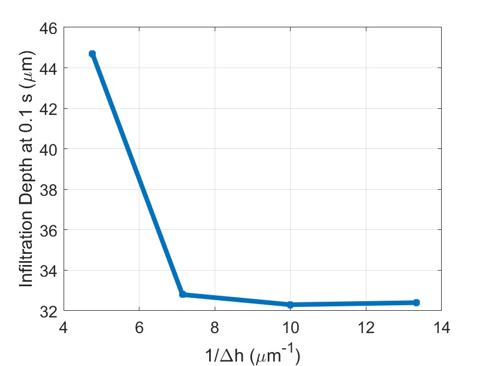
\includegraphics[width=\linewidth]{Figures/infilDepthMesh.png}
    \caption{Infiltration Depth ($\mu m$) as a function of the inverse of representative mesh size ($\mu m ^{-1}$)}
    \label{fig:meshSensResults}
\end{figure}

\begin{table}[htp!]
    \centering
    \caption{Mesh Sensitivity Results from Fig. \ref{fig:meshSensResults}}
    \begin{tabular}{c|c}
       Representative Mesh Size (m)  & Infiltration depth at 0.1 s (m) \\
       \hline
        $2.1\times10^{-07}$ & $4.475\times10^{-05}$ \\
        $1.4\times10^{-07}$ & $3.281\times10^{-05}$ \\
        $1.0\times10^{-07}$ & $3.232\times10^{-05}$ \\
        $7.5\times10^{-08}$ & $3.238\times10^{-05}$
    \end{tabular}
    \label{tab:meshSensResults}
\end{table}

\subsubsection{2D CFD Model}
In Section \ref{sec:methods}, it is mentioned that the boundary conditions on the 2D model make it such that it is not strictly a capillary-driven flow, but also inertially-driven. This has unintneded consequences on the results. The limitations in the 2D model causes the flow to reach a state of equilibrium, as seen in Fig. \ref{fig:rect_v_feather}. This phenomenon is non-physical, since the CMAS should continue to infiltrate instead of reach a point of equilibrium \cite{Naraparaju2017}. So, the 2D geometry cannot be used to ``resolve'' the infiltration process. However, it is still valuable in the sense that it can demonstrate a microstructure's ability to stop the infiltration under different circumstances.

To understand the effect of geometry, the 2D CFD results from the rectangular and feathery channel geometries are shown in Fig. \ref{fig:dimensions}.
Additionally, the 2D CFD results are compared to analytical solutions of the open-pipe and concentric-pipe models (OPM, and CPM respectively) \cite{Naraparaju2019} based on models detailed in Appendix \ref{sec:app:RaviPipeModels}. 
Fig.~\ref{fig:rect_v_feather} shows the infiltration depth versus time for the rectangular and feathery simulations, co-plotted with the analytical OPM and CPM solutions. 
Note that the CFD results in Fig.~\ref{fig:rect_v_feather} account for a fluidic viscosity that varies with temperature which is based on polynomial fit to experimentally-measured data \cite{Naraparaju2017}.\\

First, consider the rectangular and feathery CFD data in Fig.~\ref{fig:rect_v_feather}.
These CFD results show that the feathery channel works to mitigate infiltration as compared to the rectangular channel. Such an inference can be drawn from the CMAS infiltrating to shallower depths for the feathery channel compared to the rectangular channel. 
% Next, consider the circular and annular CFD results in Fig.~\ref{fig:rect_v_feather}, which differ as they depict a constant value for both cases.
% These differences are associated with the CMAS flow in the circular and annular channels results reaching an equilibrium at essentially the initial condition. 
% Such a result may seem counter-intuitive at first, however, it is supported by capillary flow theory.
% Capillary flow in small tubes is driven by the inertial response time \cite{Weislogel}, $t_{R}  \thicksim \sqrt{\frac{\rho R^{3}}{\sigma}}$; since the radius of the tube is small, the inertial response time is on the order of $1\times 10^{-9} s$. This is much smaller than the minimum time-step of the CFD simulations.
% Therefore, CMAS infiltration flow reaches an equilibrium immediately.
%Experimental results \cite{Naraparaju2019} for infiltration depth versus time are compared to simulations. These experimental results come from the German Aerospace Center, and the material used for “CMAS 1” is consistent with the material defined in the simulation. Unfortunately, the data is much farther advanced in time and with much less time resolution than the simulation. 


To understand the evolution of CMAS attack, the time history of the CMAS distribution is discussed. 
The effort starts with data extracted from the CFD results. The CFD time history is plotted in Fig.~\ref{fig:rect_v_feather} and, at several points of interest in time, contour plots of the CMAS volume fraction and TBC temperature are plotted in Fig. \ref{fig:feathery_timehistory}. In the contour plots, the red/gray area shows the distribution of air and CMAS, and the red-orange gradient shows the temperature distribution within the TBC (with isocontours in intervals of 1 K). First, consider the initial infiltration in both the rectangular and feathery channels on a time interval from $t=0$ to $t=0.001 s$ in Fig.~\ref{fig:rect_v_feather}.
This early infiltration occurs much faster and the rate of infiltration appears to significantly slow down thereafter. 
Such an fast infiltration occurring early is a result of the conical shape of the micro structure in the coating, shown in Fig.~\ref{fig:feathery_timehistory}. It appears to work much like a converging nozzles, where the flow accelerates with the reduction of the cross-sectional, interstitial area. 

Now consider a later time interval range from $t=0.001 - 0.13 s$ in Fig.~\ref{fig:feathery_timehistory}.
At $t \approx 0.05s$, the infiltration rates of the rectangular and feathery channels diverge.
There, the infiltration in the rectangular channel continues at a faster rate than in the feathery channel.
At $t \approx 0.13 s$, the CMAS in the feathery channel reaches an equilibrium state and no longer infiltrates. Concurrently, the infiltration in the rectangular channel shows a trend that indicates it begins to slow down.
Lastly, after $t \approx 0.15 s$, the infiltration in the rectangular channel eventually reaches an equilibrium as well.
It is important to emphasize that the infiltration in the feathery channel reaches an equilibrium faster and penetrates to shallower depths than in the rectangular channel.
Such an observation is consistent with previous experimental results \cite{Naraparaju2017} and further demonstrates the effectiveness of feathery TBCs to resisting CMAS attack.

In further evaluation of the results, it can be observed from Fig. ~\ref{fig:feathery_timehistory} when focusing on the distribution of air and CMAS that air pockets form within the infiltrated CMAS.
With respect to this, recall that the the thermal conductivity of air is $1-2$ orders of magnitude lower than that of the TBC and CMAS (depending on the temperature). Such air pockets can also not support convection. Hence, the air pockets potentially contribute to a decrease of thermal conductivity in a TBC that has experienced CMAS attack.

In Fig.~\ref{fig:feathery_timehistory}(center) and ~\ref{fig:rect_timehistory}(center), a developing temperature profile is seen within the TBC. The temperature profile develops as energy is absorbed by the CMAS moving downward and that energy is conducted back into the TBC. 
In Fig.~\ref{fig:feathery_timehistory}(right), after further infiltration, the temperature profile switches directions along the TBC interface.
This happens because more energy is being redirected to satisfy the latent heat of fusion of CMAS. The CMAS is effectively cooling the TBC.
This effect is less drastic in Fig.~\ref{fig:rect_timehistory} because there is overall less infiltrated CMAS available for energy absorption.

One discrepancy between these results and previous work is that the meniscus of the CMAS/air interface is convex in Figures \ref{fig:feathery_timehistory} and \ref{fig:rect_timehistory}. Previous work suggests that this meniscus should be concave \cite{Naraparaju2019}. This discrepancy is likely caused by the initial condition in the CFD simulation. That is, the flow is driven by a pressure gradient and capillary action, as opposed to being driven by capillary action from the start. Another discrepancy between experiments, analytical models, and 2D CFD is that the CMAS in the 2D CFD model reaches a state of equilibrium, rather than continuing to infiltrate. This limitation could be fixed with more mesh resolution at the CMAS/Air interface so that the capillary action is properly resolved, but the numerical methods being used here do not support AMR in 2D simulations. Hence, a 3D model is necessary to properly resolve the capillary-driven part of this phenomenon. 

% \begin{figure}[h!]
%     \centering
%     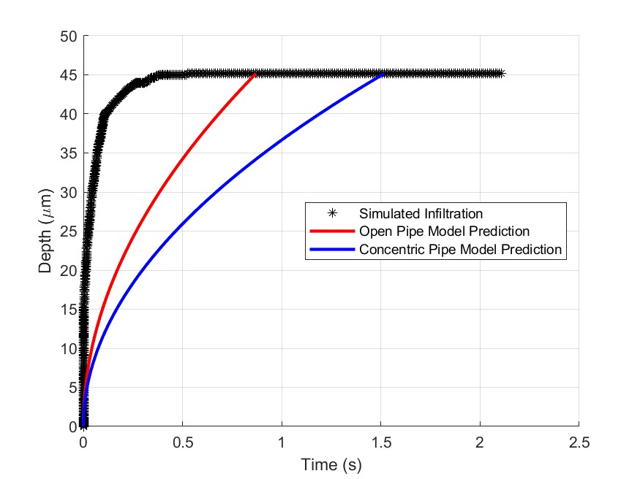
\includegraphics[width=0.75\linewidth]{Figures/analyticalBenchmark.png}
%     \caption{Comparison of Simulation Results to Analytical Models for infiltration depth}
%     \label{fig:analytBench}
% \end{figure}

\begin{figure}
    \centering
    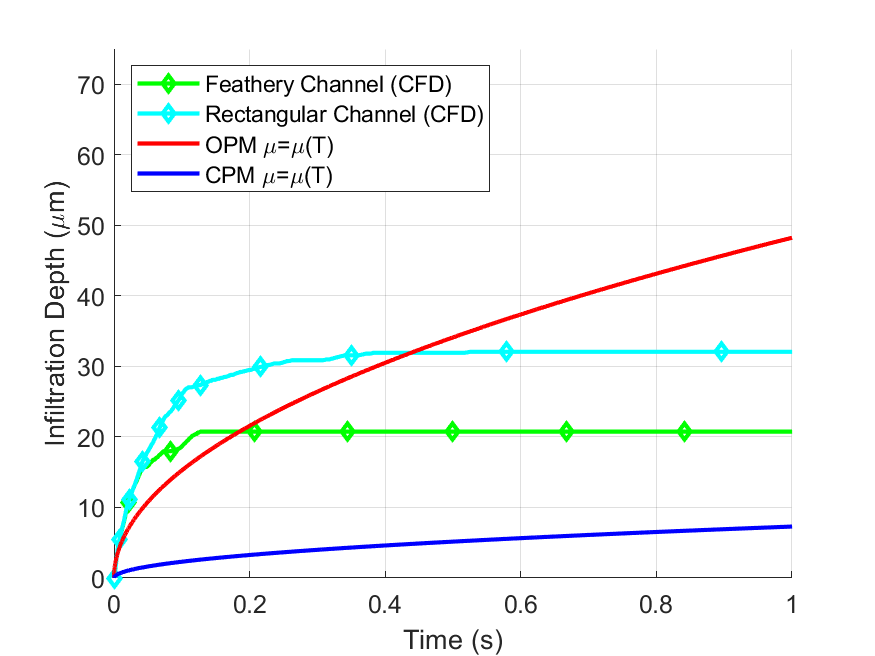
\includegraphics[width=\linewidth]{Figures/2d_results.png}
    \caption{Comparison of infiltration depth versus time for the 2D CFD model's rectangular and feathery micro-channels co-plotted with the analytical pipe model results. Note that the feathery channel reaches an equilibrium at shallower depths at a shorter time than the rectangular channel.}
    \label{fig:rect_v_feather}
\end{figure}

\begin{figure*}
    \centering
    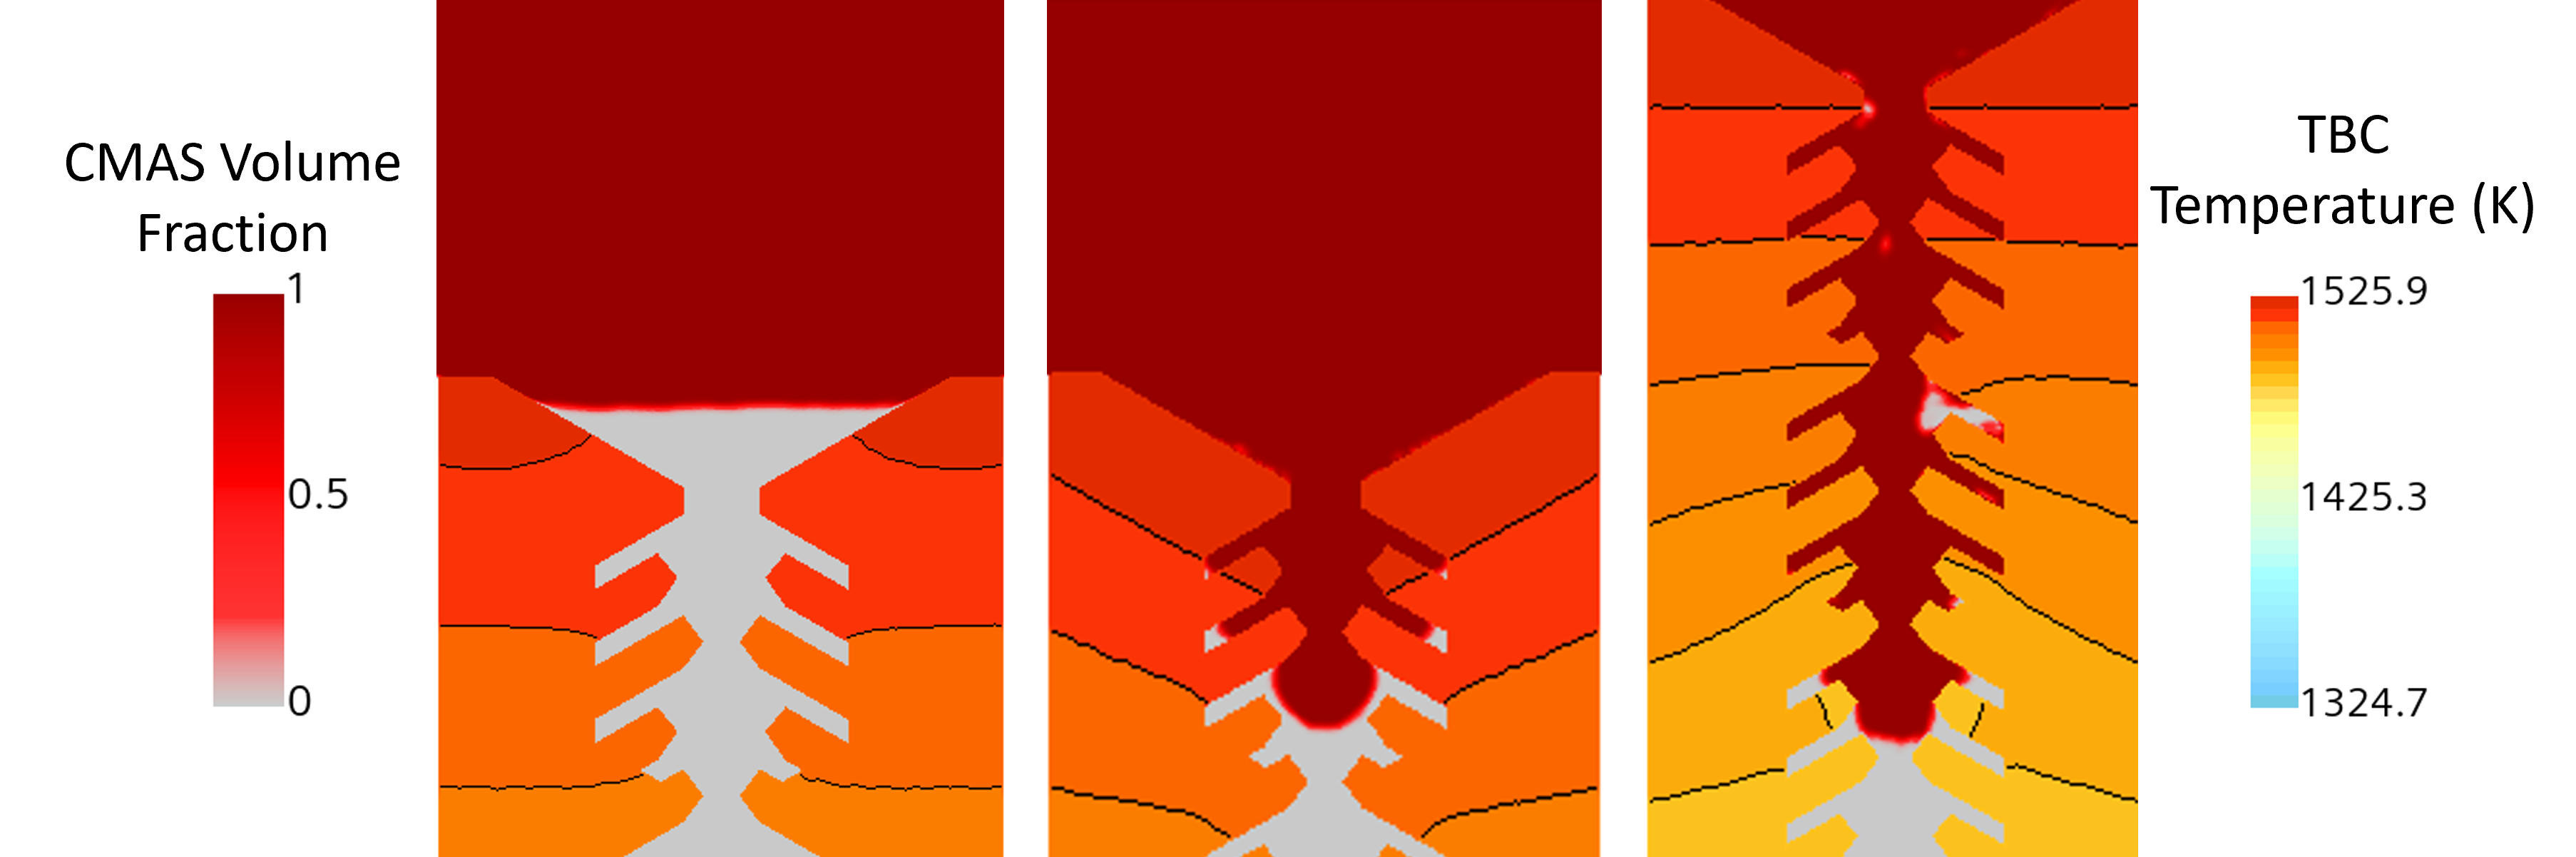
\includegraphics[width=\linewidth]{Figures/featheryTimeHistory.png}
    \caption{Time history of the feathery TBC simulation showing the volume fraction of CMAS and the temperature of the TBC (for $Oh_{initial} \approx 115$ to $Oh_{final} \approx 1300$). The left ($t \approx 2\times 10^{-5}s$) image shows the initial conical infiltration, the middle image ($t\approx 0.005 s$) shows CMAS as it infiltrates the feather arms, and the right image ($t \approx 0.13 s$) is the equilibrium point. Note that the isolines in the TBC represent the thermal gradient, where the temperature at each isoline is 1 K less than the one above it.}
    \label{fig:feathery_timehistory}
\end{figure*}

\begin{figure*}
    \centering
    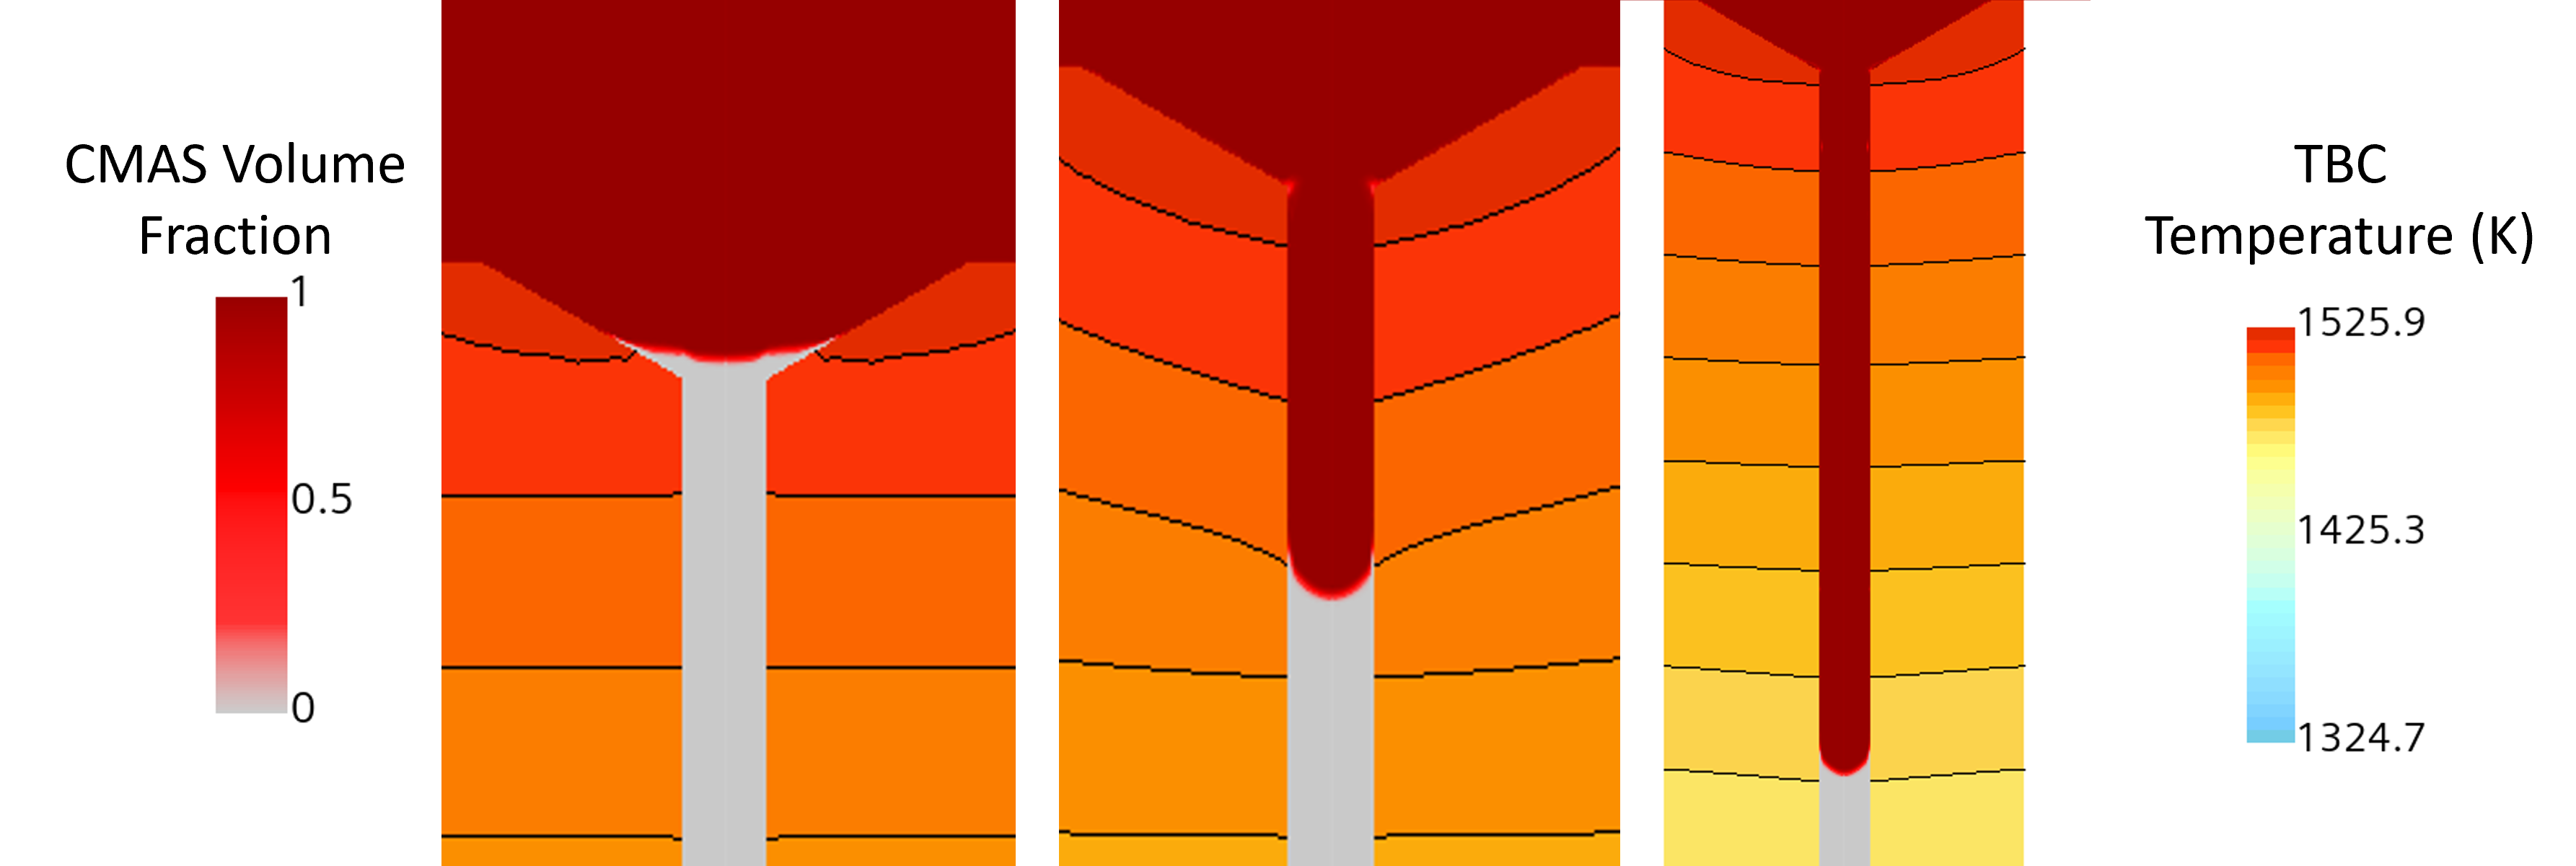
\includegraphics[width=\linewidth]{Figures/rect_timeHistory.png}
    \caption{Time history of the rectangular TBC simulation showing the volume fraction of CMAS and the temperature of the TBC (for $Oh_{initial} \approx 115$ to $Oh_{final} \approx 1300$). The left image ($t \approx 1\times 10^{-5}s$) shows the initial conical infiltration, the middle image ($t \approx 0.1 s$)shows CMAS as it infiltrates the thin rectangular channel, and the right image ($t \approx 0.4 s$) is the equilibrium point. Note that the isolines in the TBC represent the thermal gradient, where the temperature at each isoline is 1 K less than the one above it.}
    \label{fig:rect_timehistory}
\end{figure*}

% The results from the experiments, pipe models, and the simulation are summarized in Table \ref{tab:resultsSummary}.

% \begin{table}[htp!]
%     \centering
%     \caption{Summary of Analytical, Numerical, and Experimental Results. Note that the simulated result is extrapolated to the same time as the experiments and models, because the simulation result is asymptotic at t = 0.5 s}
%     \begin{tabular}{c|c|c}
%        -  & Time (s) & Depth ($\mu m$)\\
%        \hline
%         Experiment & 120 & 125\\
%         Open-pipe & 120 & 176\\
%         Closed-pipe & 120 & 95\\
%         rectangular micro-channel Simulation & 120 & 45 (extrapolated) \\
%         Feathery micro-channel Simulation & 120 & 45 (extrapolated)
%     \end{tabular}
%     \label{tab:resultsSummary}
% \end{table}

% \noindent Fig.\ref{fig:ODEvSim_Oh_nonconstant} shows how system of ODEs is solved, and compared to the simulation data. Here, the analytical solution for capillary flow in a "feathery" micro-channel and the simulated solution for the same flow agree fairly well. An important note is that to attain this good agreement, the Ohnesorge number was linearly increased at each timestep in the solution of the ODE system. This was meant to replicate the linearly increasing viscosity, and eventual solidification, of the particle in the channel. This is important because it provides further evidence that capillary flow is not the only dominant feature in the infiltration of CMAS into a TBC.

% \begin{figure}[htp!]
% \centering
% 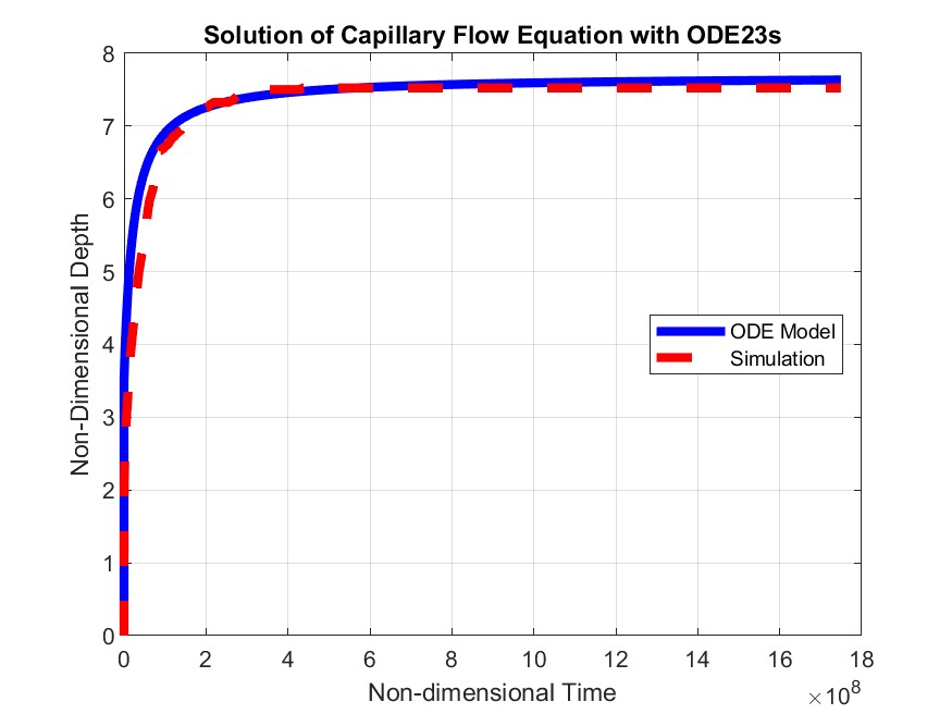
\includegraphics[width=.7\linewidth]{Figures/ODEsolution.png}
% \caption{Comparison of simulation and analytical infiltration depth versus time (non-dimensional).}
% \label{fig:ODEvSim_Oh_nonconstant}
% \end{figure}

\subsubsection{3D CFD Model}

While the 2D model was unable to attain spontaneous capillary flow, the CMAS in the 3D model was able to spontaneously form a meniscus, and infiltrate the TBC without the assistance from an external pressure gradient. Hence, this model can reasonably resolve the actual physical processes in the CMAS infiltration, rather than just a comparison tool like the 2D model. 

The infiltration depth as a function of time for the 3D model is shown in Fig. \ref{fig:3D_results}. The reults from the 3D model, 2D models, OPM, and CPM are compared. Fig. \ref{fig:3D_results} shows that the CMAS in the 3D CFD model does not reach a point of equilibirum, as the 2D CFD does, and the shape of the infiltration versus time curve is similar to that of OPM and CPM. 

\begin{figure*}
    \centering
    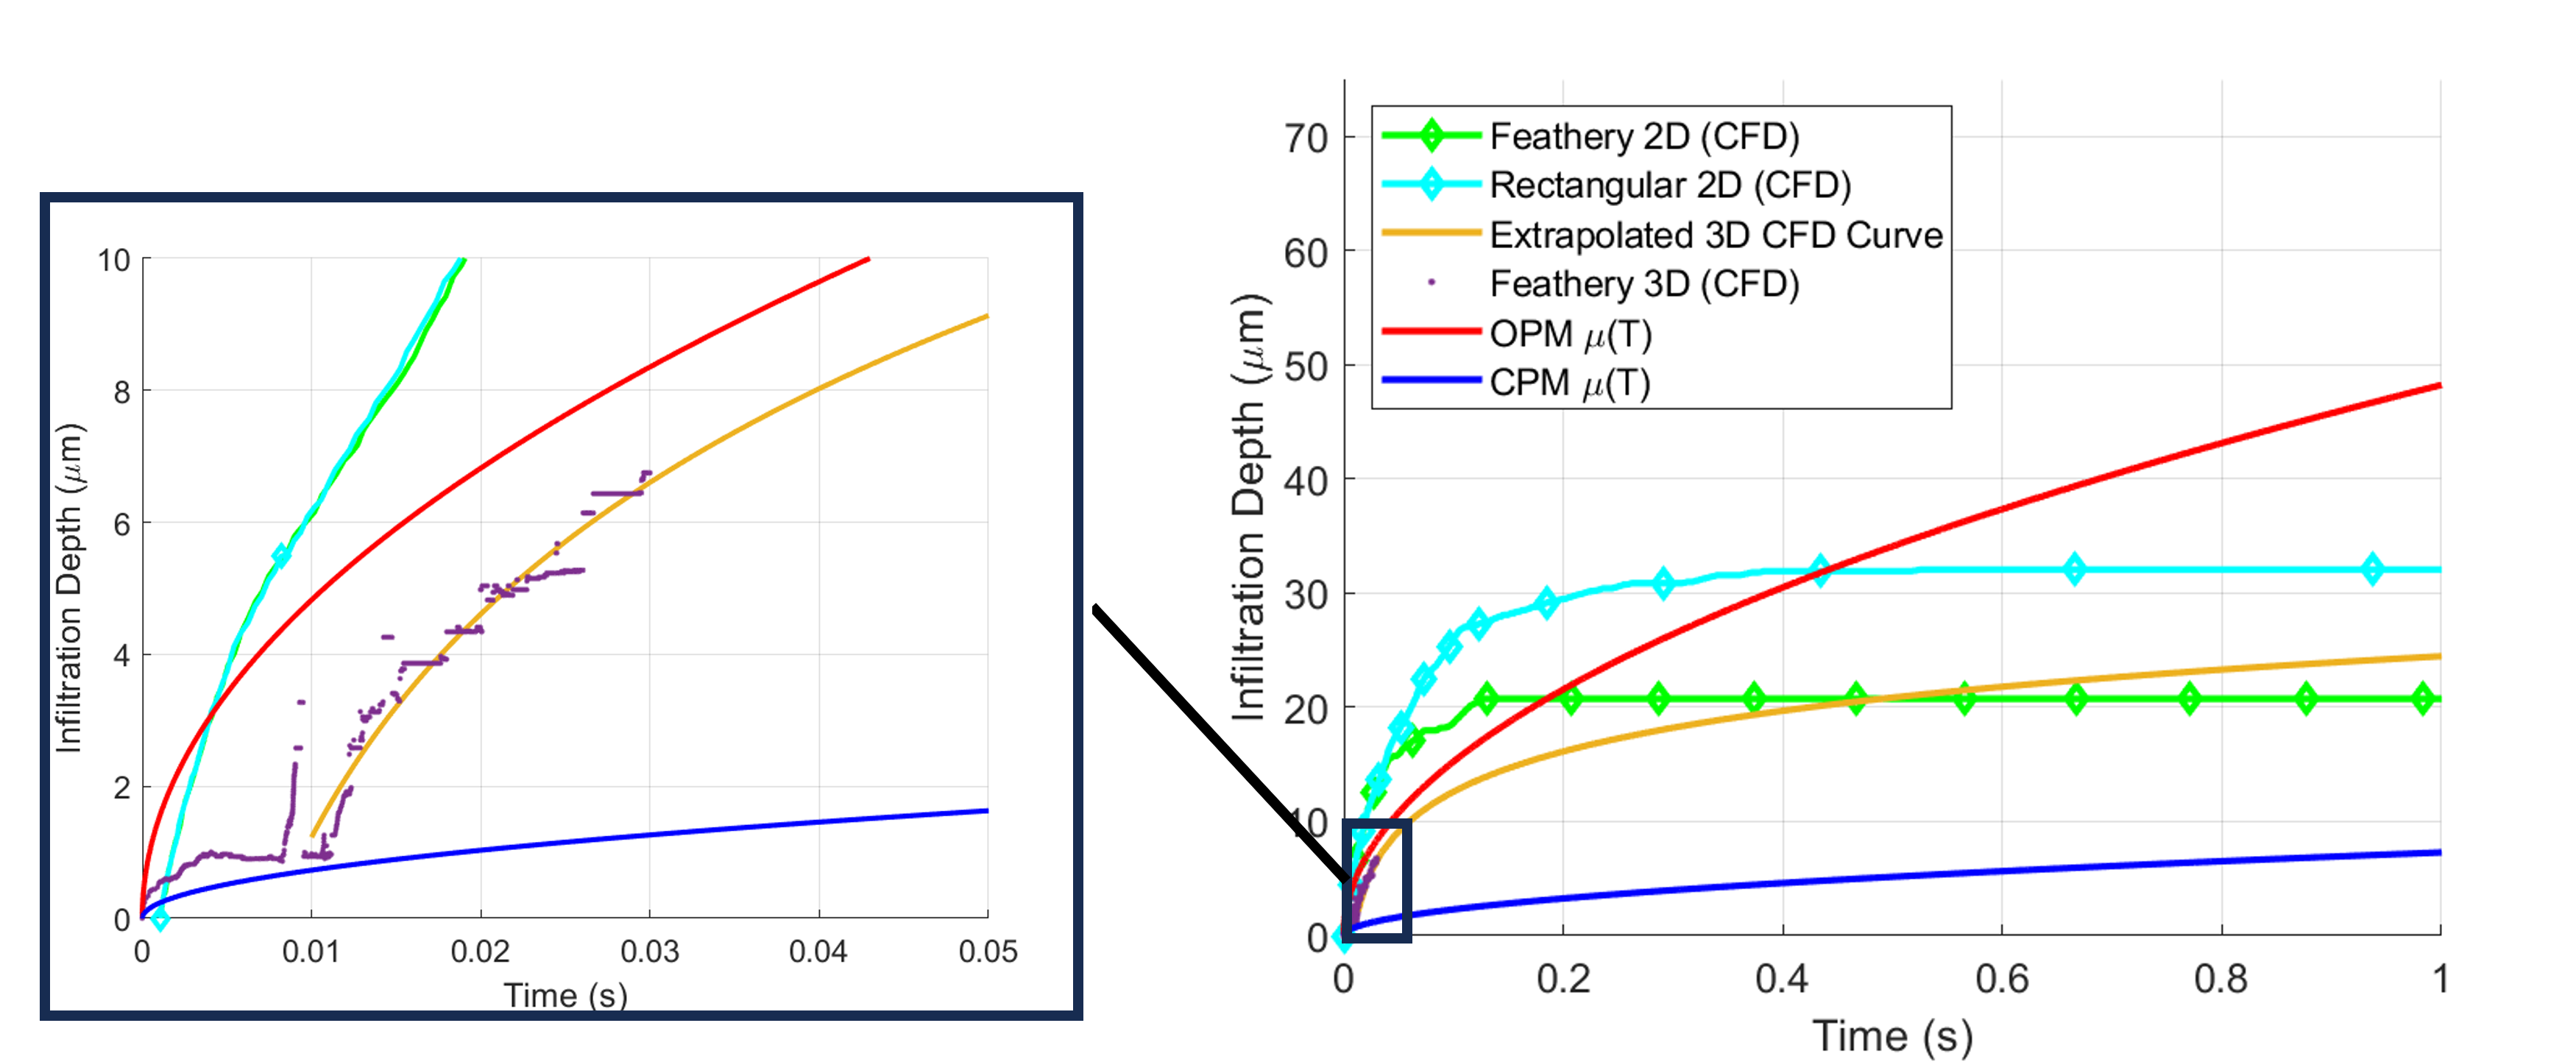
\includegraphics[width=\linewidth]{Figures/3D_results.png}
    \caption{Infiltration depth versus time for the 3D CFD model. Here, the simulation data is plotted along with a curve-fit of that data in order to extrapolate past the simulated time.}
    \label{fig:3D_results}
\end{figure*}

The time resolution of experimental measurements is very low, with measurements taking place every few minutes during infiltration \cite{Naraparaju2017}. The first data point that can be compared to is taken at 120 s. One drawback of the 3D CFD model is the time it takes to run. Even on an HPC system using 4 Intel Xeon Platinum 8558 processors (192 compute cores), it still takes nearly a week to run the 3D CFD model to 0.1 s of physical time. As a result of this, to compare to experiments, the 3D CFD infiltration versus time data must be fitted to a curve, and the depth at 120 s must be extrapolated to compare to the experiments. The fitted curve is shown in Fig. \ref{fig:3D_results}, and the extrapolated depth at 120 s is shown in Table \ref{tab:resultsCompare}. Note that the time-period where the meniscus was forming was excluded from the curve-fit. The extrapolated depth of the 3D CFD model at 120 s is ~50 $\mu m$. So, the 3D CFD model under-predicts the infiltration depth compared to all other models. This under-prediction can be partially explained by the 

\begin{figure*}
    \centering
    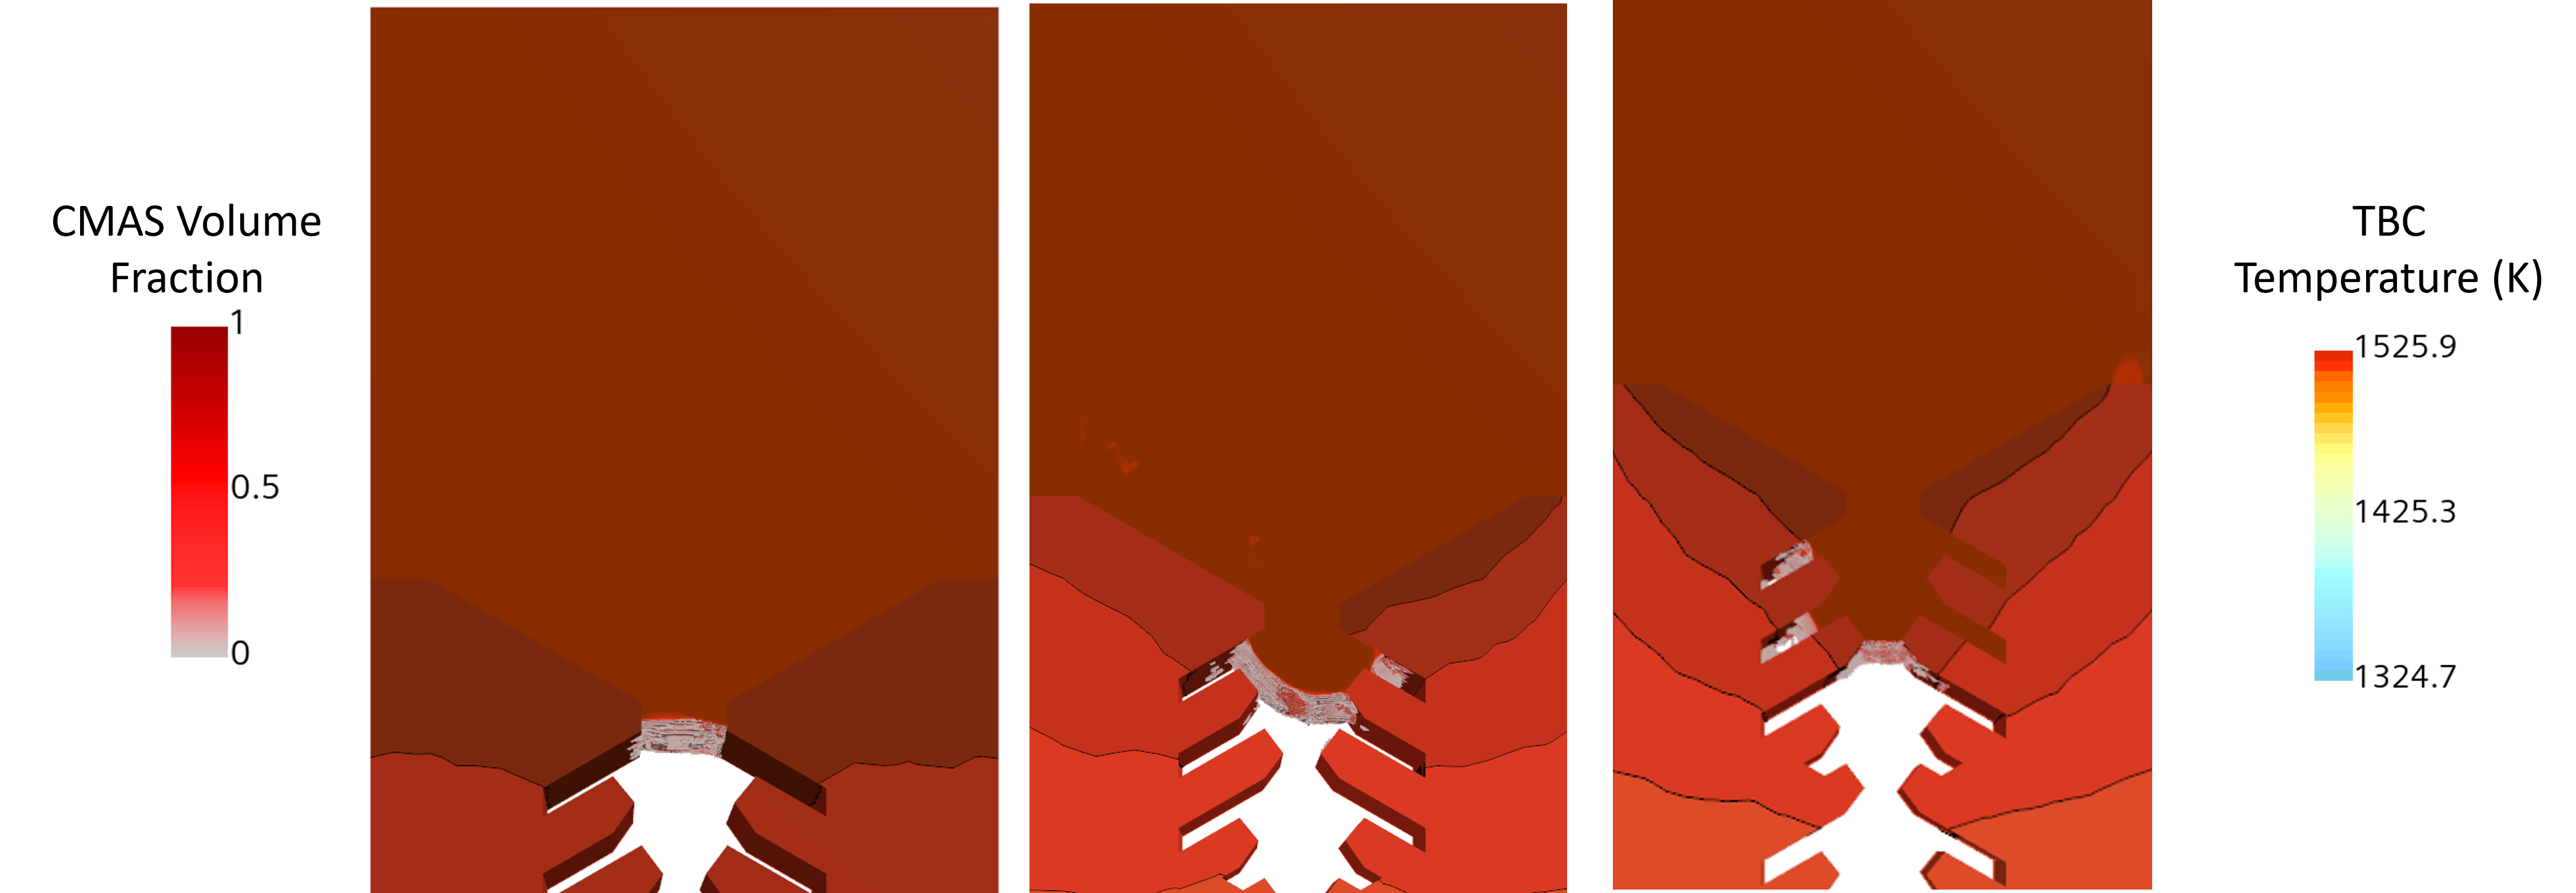
\includegraphics[width=\linewidth]{Figures/3D_timehistory.png}
    \caption{Time history of the feathery 3D CFD model showing the volume fraction of CMAS and the temperature of the TBC. The left image ($t \approx 1\times 10^{-3}s$) shows the initial infiltration, where the meniscus begins to spontaneously form, the middle image ($t \approx 0.12 s$) shows the CMAS as it begins to enter the first feather gap, and the right image ($t \approx 0.035 s$) shows the CMAS as fully infiltrating the feather arms, and continuing to move down the TBC. Note that the isolines in the TBC represent the thermal gradient, where the temperature at each isoline is 1 K less than the one above it.}
    \label{fig:3D_timehistory}
\end{figure*}

Importantly, the prediction from the extrapolated curve is in between the results from OPM and CPM in Fig. \ref{fig:3D_results}. Experimental measurements at 120 s are also between the predictions for OPM and CPM \cite{Naraparaju2017}. So, the 3D CFD model is more closely aligned with experimental results than the present theoretical models. This is beneficial because it allows more accurate predictions, but since the 3D CFD model is so computationally expensive, it is worth looking for a simpler model, such as FPNM. However, this is only the case at small time scales. At larger timescales, the 3D CFD model under-predicts the infiltration, as seen in Table \ref{tab:resultsCompare}. 

Fig. \ref{fig:3D_timehistory} shows images of the CMAS infiltration at several important time points. Fig. \ref{fig:3D_timehistory} (left) shows the meniscus spontaneously forming, and the CMAS beginning to move downward from its original state. Then, Fig. \ref{fig:3D_timehistory} (center) shows the CMAS starting to enter the feather gaps as it creeps along the TBC walls. Interestingly, in Fig. \ref{fig:3D_results}, there are brief pauses in the infiltration (like between $t=0.015 s and t=0.0175 s$). These pauses seem to correlate periods where the flow in the primary gap stops, but the flow in the feather gaps continues. The flow must reach a certain point in the feather gap for the CMAS to continue to infiltrate the primary channel. This phenomena occurs between the timepoints in Fig. \ref{fig:3D_timehistory} (center) and Fig. \ref{fig:3D_timehistory} (right).

\subsection{FPNM: Benchmarks with CFD, Conventional Models, and Experiment}
%Comparison of analytic and CFD results to evalaute analytic model accuracy. 
Consider infiltration comparisons of the newly formulated FPNM model to results from the OPM, CPM, and the CFD models. 
Results are plotted in Fig. \ref{fig:pipeNetworkResults}, with comparisons of FPNM (Eq.~\ref{eq:FPNM_dimensional}), OPM (Eq.~\ref{eq:oPM}), and CPM (Eq.~\ref{eq:CPM}). The CFD results are based on the model described in Fig.~\ref{fig:rect_v_feather}. 
The FPNM infiltration was calculated with both constant viscosity ($\mu = 5.65$ Pa$\cdot$s) and temperature-dependent viscosity, while OPM and CPM were only calculated with constant viscosity.
In the early stages of this comparison $(t<0.025s)$, it can be observed that the FPNM provides an improved correlation with the CFD results compared to the OPM and CPM models. The improved agreement is observed in the initially rapid infiltration rate from the FPNM. 
As time evolves to $t\approx0.5s$, the FPNM tends to be more in-line with OPM and CPM. The CFD model results shows an equilibrium infiltration depth, whereas the FPNM, OPM, and CPM results indicate that equilibrium is not achieved. 
Additionally, at times beyond $0.5s$, the FPNM also appears to be bounded by the OPM and CPM results. 
To summarize the results, the three model results at $120 s$, and a measured experimental result are summarized in Table \ref{tab:resultsCompare}. The CFD results are not included in this table because the infiltration equilibrates in the CFD, so the results are not directly comparable.
Table \ref{tab:resultsCompare} shows that the experimentally measured infiltration is also bounded between OPM and CPM.
However, FPNM is closer to the experimental result than OPM. 
Thus, the results demonstrate that the FPNM enhances the predictions of infiltration depth for CMAS attack.

One aspect the FPNM does not take into account is the solidification of the CMAS. As the CMAS approaches the solidification onset temperature, it will tend to slow down not just due to an increase in viscosity, but because the CMAS itself will begin to crystallize \cite{Naraparaju2019}. This process occurs beyond what is calculated in Fig.\ref{fig:pipeNetworkResults} for FPNM, OPM, and CPM. However, this shows that FPNM is over-predicting the infiltration depth. If a solidification model were included in FPNM, it would align even closer to experimental results.

Another advantage of the FPNM is its computational efficiency. While it is not as efficient as a purely algebraic model, like OPM or CPM, it is far more efficient than a fully-fledged CFD model. The computational time required to solve the FPNM equation is on the order of minutes whereas the CFD models could take hours for a 2D model or days for a 3D model. Thus, the FPNM is a compromise between the speed of OPM/CPM, and the accuracy of CFD. The speed of FPNM also allows for quick evaluation of different material properties. The ability to solve FPNM incrementally also allows the addition of additional non-linear steps to the solver, such as solidification, or other temperature-dependent properties. The speed of FPNM could be further optimized using parallelization. 



%Fig. \ref{fig:pipeNetworkResults} shows how the analytical solution to the ODE described in Section \ref{sec:pipeNetworkMethod} compares to the analytical solution from the open and concentric-pipe models, as well as the simulated results for the feathery and rectangular channel flow. Here, it is seen that the pipe network model more closely resembles the simulated results at the beginning of the infiltration; the simulated results and pipe network both infiltrate much quicker than the open and concentric-pipe models at first. As the infiltration continues however, the pipe network result does not change as sharply as the simulated result, and also does not equillibrate. Results for infiltration depth at 120 s for all three analytical models are summarized in Table \ref{tab:resultsCompare}. Table \ref{tab:resultsCompare} and Fig. \ref{fig:pipeNetworkResults} show that the result from the pipe network model becomes bounded between the open-pipe and concentric-pipe models. Therefore, the pipe-network model is more in-line with experimental results than the open-pipe and concentric-pipe models \cite{Naraparaju2019}. 

\begin{figure}[htp!]
    \centering
    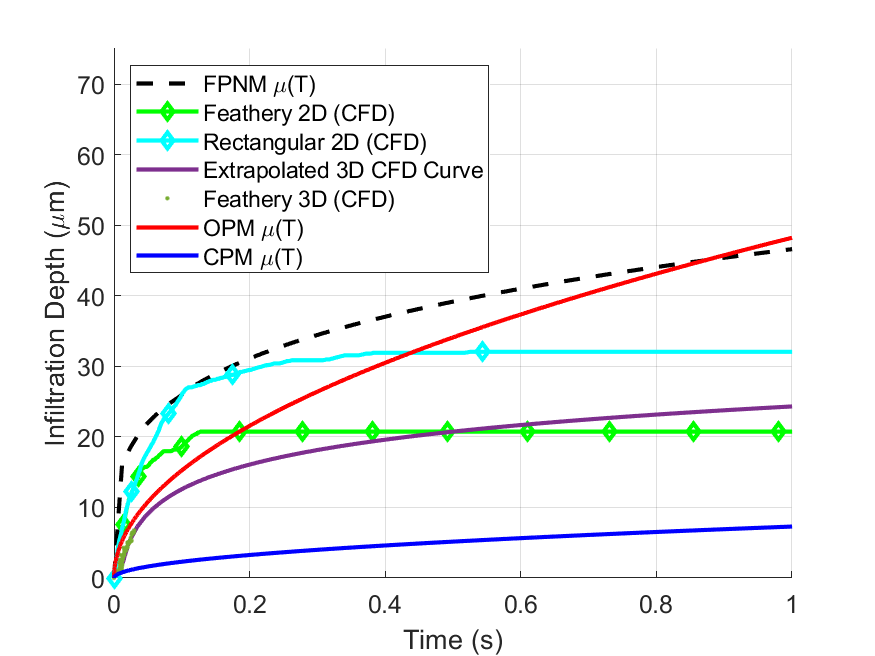
\includegraphics[width=\linewidth]{Figures/analytical.png}
    \caption{Depth versus time for the CFD, analytical pipe models, and the proposed FPNM (with both a constant viscosity and temperature-varying viscosity solution).}
    \label{fig:pipeNetworkResults}
\end{figure}

\begin{table}[htp!]
\caption{\label{tab:resultsCompare} Infiltration depth at 120 s from experiments \cite{Naraparaju2019}, open-pipe \cite{Naraparaju2019}, concentric-pipe \cite{Naraparaju2019}, and feathery pipe network model}
\centering
\begin{ruledtabular}
\begin{tabular}{lcc}
 & Infiltration Depth ($\mu m$)\\
\hline
Experiment & 125\\
Open-pipe & 176\\
Concentric-pipe & 95\\
Feathery Pipe-Network Model & 154\\
3D CFD Model & 50
\end{tabular}
\end{ruledtabular}
\end{table}

\subsection{Geometric Parameterization with FPNM}

The quick solutions offered by FPNM (the ODE can be solved in minutes, whereas CFD can take hours or days) allows for easy manipulation of geometric parameters without the need to change a physical model, remesh, and rerun the solution every time. Hence, it is advantageous to use FPNM to study how the geometric parameters of the TBC affect the CMAS infiltration.

First, the affect of the intercolumnar gap, $B$, was analyzed, and the results are shown in Fig. \ref{fig:columnGapStudy}. 
Here, it is shown that larger intercolumnar gaps lead to faster infiltration, and this effect scales nonlinearly, meaning larger gaps allow exponentially faster infiltration. 
This data is supported by other's numerical efforts evaluating the TBC microstructure \cite{Sirigiri2018}.
A good analogy to describe why this physically makes sense is blood flow. When arterioles and venules bifurcate and becomes smaller, their flow-resistance becomes larger, because the resistance is inversely proportional to $R^{4}$ \cite{Chandran2012}. So, it can be said that smaller intercolumnar gaps increase the TBC's resistance to infiltration.

\begin{figure}[htp!]
    \centering
    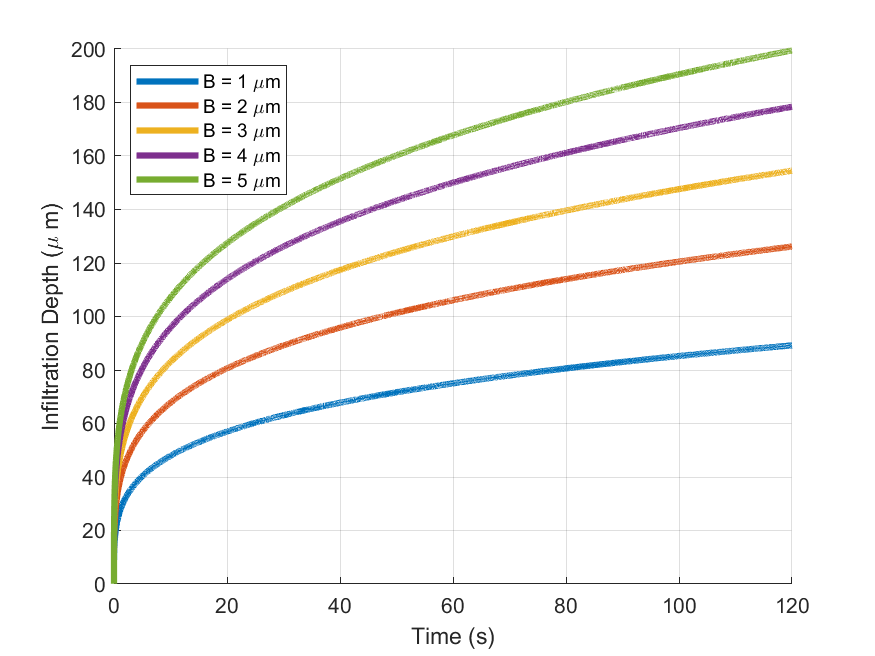
\includegraphics[width=\linewidth]{Figures/intercolumnarGapStudy.png}
    \caption{Depth versus time for various intercolumnar gap widths using FPNM.}
    \label{fig:columnGapStudy}
\end{figure}

Similarly, the feather gap width, $b$, was evaluated, and results are shown in Fig. \ref{fig:featherGapStudy}. 
Here, larger feather gaps lead to faster overall infiltration in the primary channel, because the CMAS must fully infiltrate the feather gaps before it can move further down the primary channel. Hence, increasing the flow resistance at the feather gap increases the overall resistance. 
However, decreasing the feather gap width had diminishing returns, after $b = 2 \mu m$, the infiltration is not mitigated nearly as much as before $b=2 \mu m$.

\begin{figure}[htp!]
    \centering
    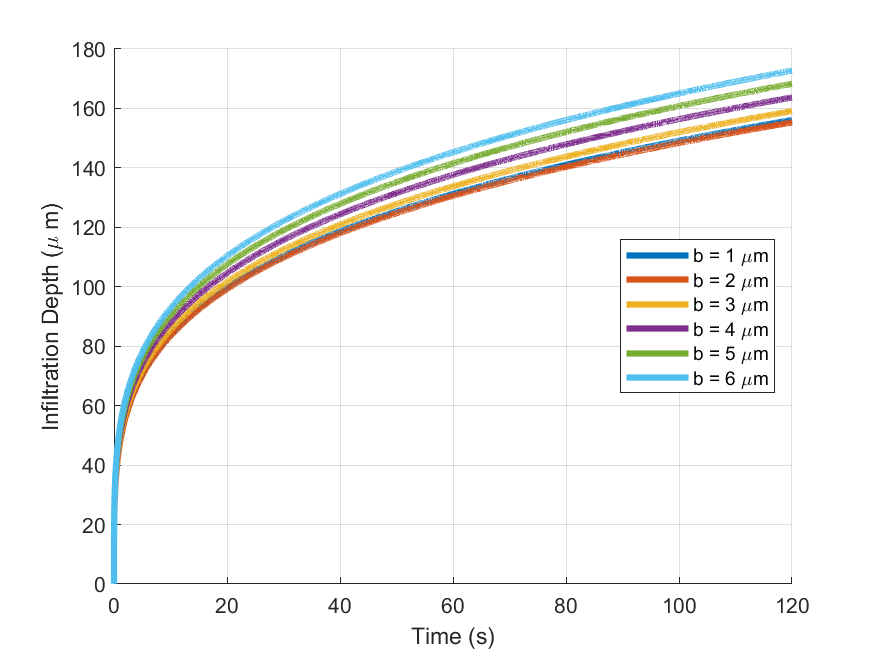
\includegraphics[width=\linewidth]{Figures/featherGapStudy.png}
    \caption{Depth versus time for various feather gap widths widths using FPNM.}
    \label{fig:featherGapStudy}
\end{figure}

The results in Fig. \ref{fig:columnGapStudy} and Fig. \ref{fig:featherGapStudy} elucidate an important ratio,  $B^{*} = B/b$. As $B^{*}$ increases, the infiltration will become slower. Designing TBC microstructures around this ratio will lead to more effective infiltration mitigation.

The feather angle can also influence the infiltration characteristics. Infiltration depth versus time for several feather angles are shown in Fig. \ref{fig:angleStudy}. It is shown that larger feather angles tend to increase the infiltration speed, while smaller angles decrease the infiltration speed. However, increasing the feather angle has a greater effect than decreasing it.

\begin{figure}[htp!]
    \centering
    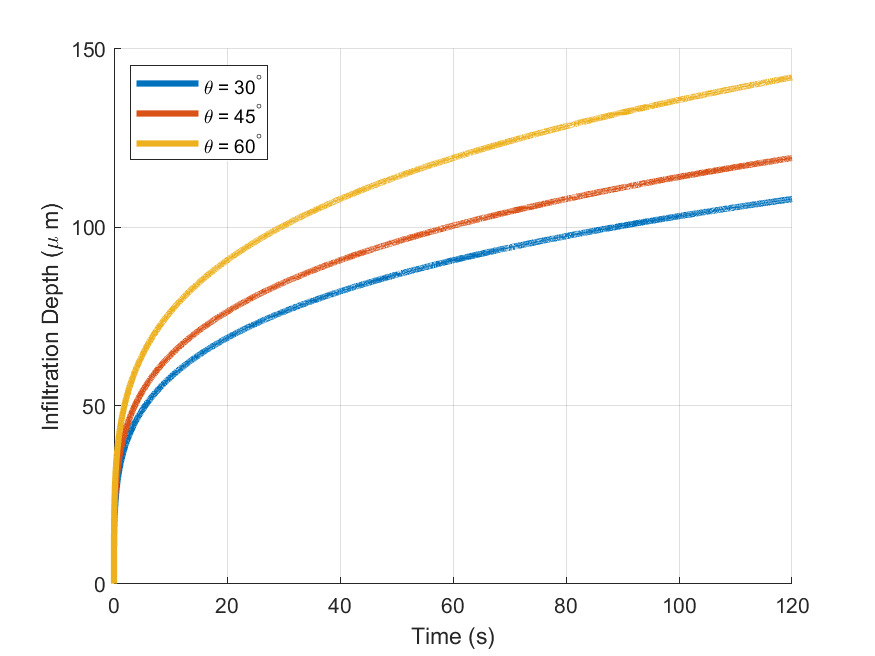
\includegraphics[width=\linewidth]{Figures/featherAngleStudy.png}
    \caption{Depth versus time for various feather angles widths using FPNM.}
    \label{fig:angleStudy}
\end{figure}

\subsection{Characterization Based on Ohnesorge Number with CFD and FPNM}

In an effort to better understand micro-scale flows, we look at a more generalized fluid flow in the microstructures shown in Fig. \ref{fig:dimensions}. We are particularly interested in whether bringing the feathery microstructure into the broader world of microfluidics has any desirable effects. For this effort, the effect of viscosity and surface tension are evaluated. These are captured in the Ohnesorge Number, ($Oh$), a dimensionless number that represents the ratio of the viscous forces to the inertial and interfacial forces ($Oh = \mu / \sqrt{\rho \sigma L}$). 
The rectangular and feathery micro-channel simulations were reevaluated, replacing the experimentally measured viscosity with a constant viscosity, while the surface tension was held constant.
Similarly, different $Oh$ were used as inputs for FPNM.
Note that constant viscosity would not be a great assumption for the CMAS/TBC problem. However, the goal here is to generalize the approach for potential applications outside of CMAS infiltration in TBCs.
To provide some context, the CMAS in a simulation with the temperature-dependent viscosity would vary from 
$Oh\approx 10$ at the initial condition to $Oh \approx 100$ at its maximum depth. So this analysis allows evaluation of materials outside of that range.
Hence, a range of $Oh$ were evaluated to understand how $Oh$ affects the infiltration time in the CFD model, and FPNM. 
Fig. \ref{fig:rect_v_feather_oh} plots the non-dimensional equilibrium point (where $D^{*} = D/b$, $b$ is the columnar gap width) against infiltration depth for various $Oh$. 
An interesting result is that, at lower $Oh$, the rectangular micro-channel is more effective at inhibiting fluid flow, but around $Oh=500$, this trend switches, and the feathery microstructure becomes more effective. Additionally, at low $Oh$, there is also a very high sensitivity to the input $Oh$.  
From these studies, we see that the feathery structures are not always most effective and that there are regions where viscosity and surface tension parameters can play a critical role in two-phase flow in different microstructure geometries. 

\begin{figure}[htp!]
    \centering
    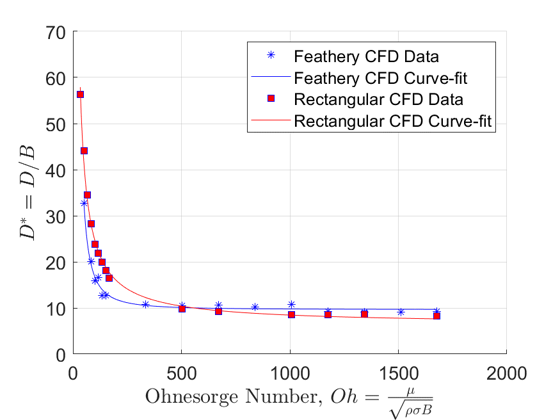
\includegraphics[width=\linewidth]{Figures/Rect_feather_compare.png}
    \caption{Non-dimensional equilibrium depth versus $Oh$ for the rectangular and feathery micro-channels using the CFD model. At lower $Oh$, the feathery microstructure allows the molten liquid to infiltrate further than the rectangular channel. However, around $Oh = 500$, this switches, and the feathery channel is more effective at stopping infiltration.}
    \label{fig:rect_v_feather_oh}
\end{figure}

Fig. \ref{fig:FPNM_Oh} shows how the infiltration as a function of time is affected by $Oh$ in FPNM. Here, it is shown that as viscous effects begin to dominate the infiltration process, the liquid tends to infiltrate slower. However, as surface tension dominates the flow, the liquid tends to infiltrate faster. Hence, the viscosity of the liquid acts as a resistive force, impeding infiltration whereas the surface tension acts as a compliant force, allowing infiltration.

\begin{figure}[htp!]
    \centering
    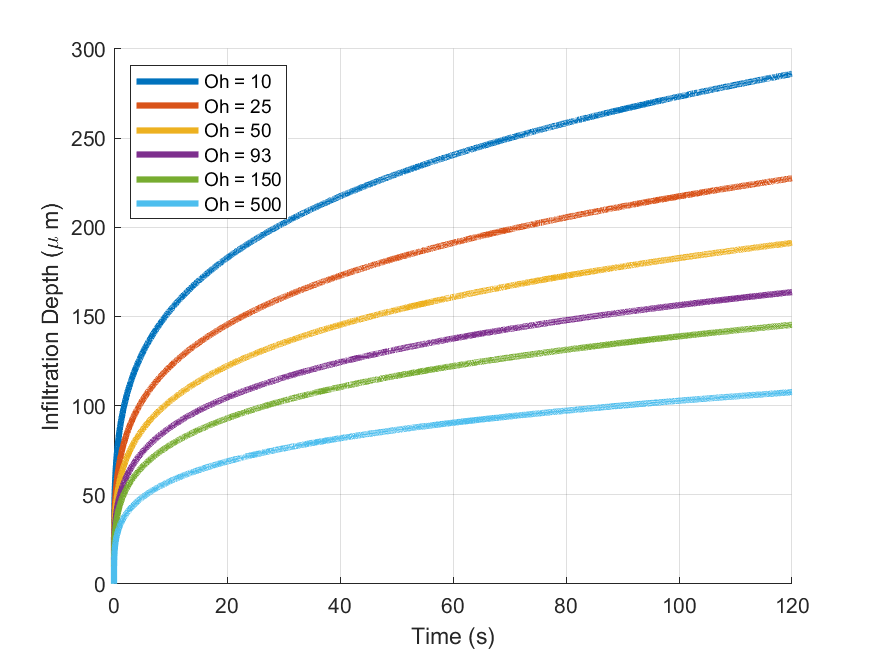
\includegraphics[width=\linewidth]{Figures/OhStudy.png}
    \caption{Infiltration depth versus time with various $Oh$. Constant viscosity FPNM was used for each calculation.}
    \label{fig:FPNM_Oh}
\end{figure}

\subsection{Characterization Based on Solidification}
\label{sec:solidificationCharacterization}
The effort now moves to evaluate the effect of solidification on the infiltration time.
Such studies are developed using simulations that have an experimentally-measured viscosity (see Table~\ref{tab:CMAS and TBC properties}\cite{Naraparaju2017}), which couples to the solidification model described in Eq.~\ref{eq:solidificationModel}. In Fig.~\ref{fig:solidification}, are extracted the infiltration depth versus time for both the feathery and rectangular channels. 
To evaluate the sensitivity of the flowability threshold (FT), the parameter was varied in each simulation.  and Fig.~\ref{fig:solidification} compares these results to the result without solidification.

\begin{figure}[htp!]
    \centering
    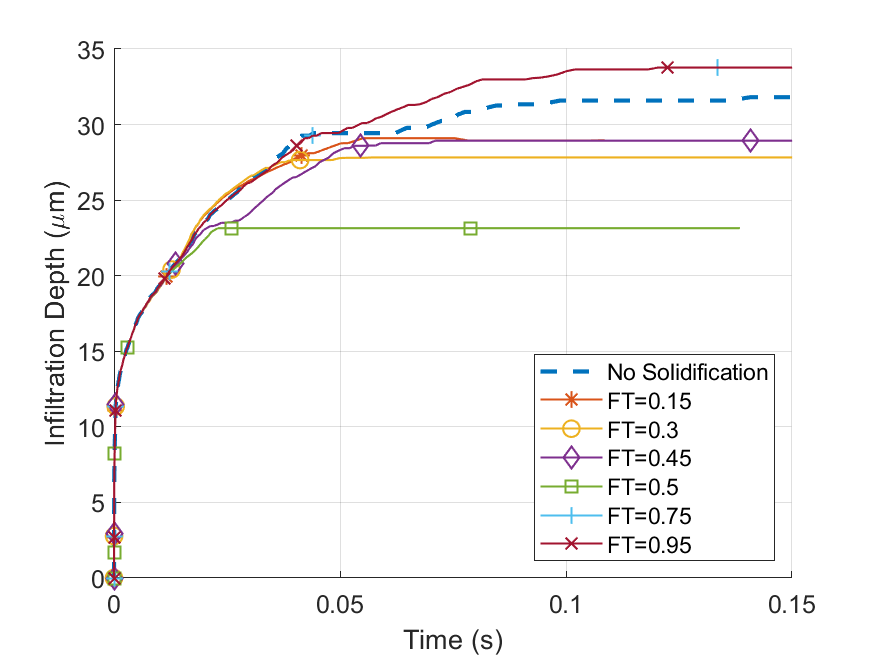
\includegraphics[width=\linewidth]{Figures/solidificationStudy.png}
    \caption{Infiltration depth versus time for the feathery and rectangular micro-channels with solidification (using a range of flowability thresholds) compared to no solidification.}
    \label{fig:solidification}
\end{figure}

Further evaluation of Fig. ~\ref{fig:solidification} demonstrates the clear character that $FT$ affects both the equilibrium depth and the equilibrium time. 
The Infiltration with the low $FT$ values (i.e., $FT=0.015$) tends to behave similarly to infiltration without solidification. 
Interestingly, as $FT$ increases, the infiltration follows a less clear, non-monotonic pattern. 
That is, the equilibrium depth for larger $FT$ cases indicated 
%either be deeper or 
shallower equilibrium infiltration depths as compared to no solidification, but the response does not indicate a monotonic reduction in the depth as $FT$ decreases. 
For example, the infiltration profile for $FT=0.75$ and $FT=0.95$ are very similar.
Such overlap suggests that after some threshold is crossed, the result will not change (i.e., the effect is saturated). 
It is interesting to point out that these cases also have a longer time to equilibrium and equilibrate at the deepest infiltration depths. 
In general, as the $FT$ value decreases, solidification appears to decrease the infiltration depth. 
Note that not including solidification may most desirable as it provides a good measure of a conservative, ``worst-case scenario'' and therefore aims to approximately bound the infiltration depth without input uncertainty associated with $FT$.

 \subsection{Characterization Based on Temperature Gradient}

A key property of a TBC is its ability to reduce the temperature between the hot engine flow, and the substrate material. So, TBCs with different temperature gradients between the top and bottom would offer varying degrees of thermal protection. Now, we seek to understand how the temperature gradient in the TBC would affect the degree of CMAS mitigation ability. Both the 3D CFD model and FPNM were evaluated when under temperature gradients, $\Delta T_{x}$ of 0.1, 1, and 10 $K/\mu m$. The results from this are shown in Fig. \ref{fig:tempGrad}

\begin{figure}[htp!]
    \centering
    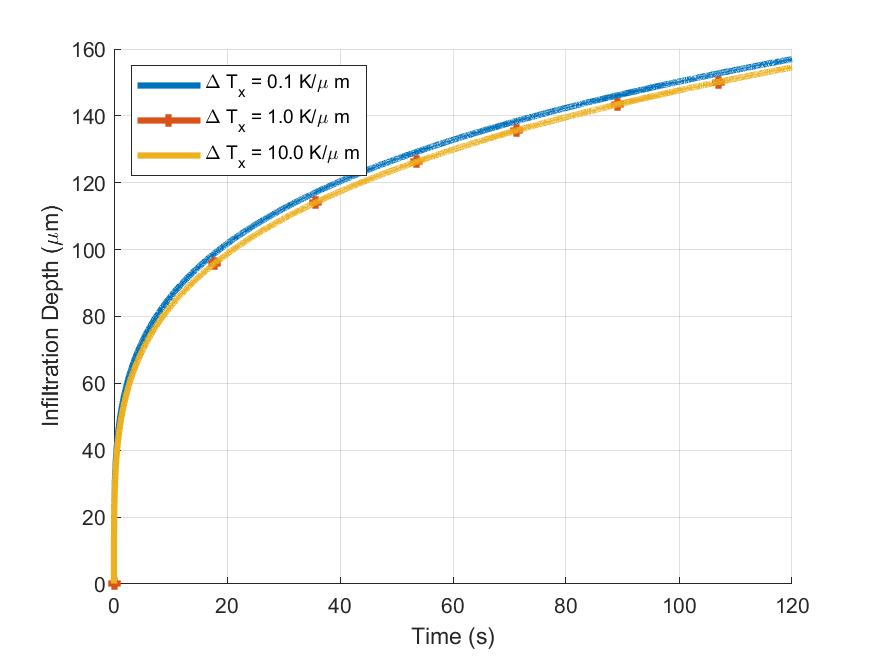
\includegraphics[width=\linewidth]{Figures/tempGradStudy.png}
    \caption{Infiltration depth versus time for the feathery micro-channels using FPNM. The temperature gradients $\Delta T = - 1 K/\mu m$ and $\Delta T = - 10 K/\mu m$ both make the CMAS reach its maximum viscosity (the temperature at which the CMAS is fully solid) very quickly, so the curves overlap.}
    \label{fig:tempGradFPNM}
\end{figure}

Fig. \ref{fig:tempGradFPNM} shows that less intense temperature gradients in the TBC lead to somewhat faster infiltration. Beyond a certain point, however, more intense temperature gradients do not lead to less infiltration. This is because maximum viscosity limit imposed on the model. Once the CMAS is considered solidified, the viscosity is no longer changing. So, if the CMAS reaches the solidification viscosity within the first few $\mu m$, then the infiltration will remain constant afterward. This is why the curves for $\Delta T_{x} = 1 K/\mu m$ and $\Delta T_{x} = 10 K/\mu m$ overlap in Fig. \ref{fig:tempGradFPNM}.


\begin{figure}[htp!]
    \centering
    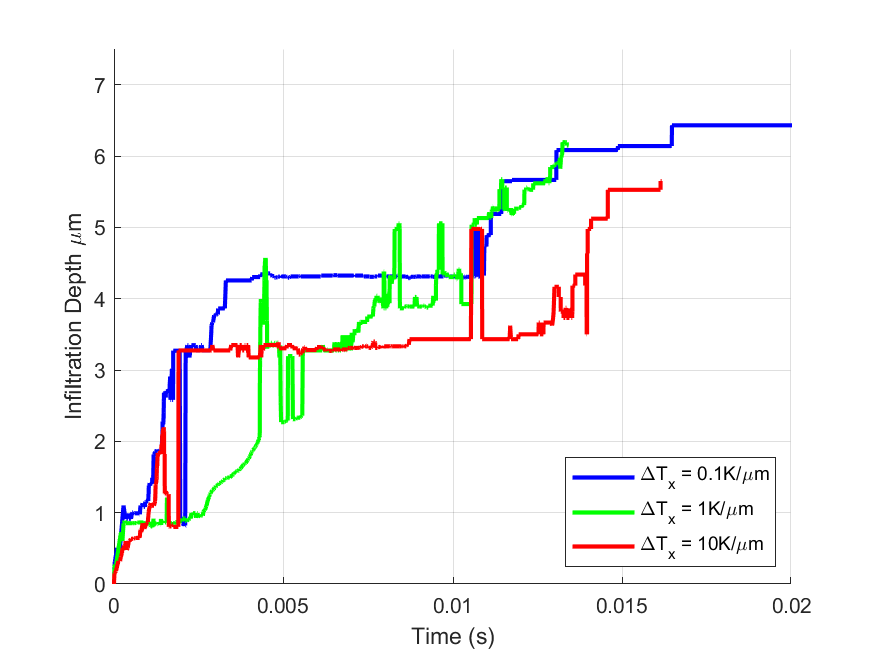
\includegraphics[width=\linewidth]{Figures/tempGradStudyCFD.png}
    \caption{Infiltration depth versus time under for the feathery micro-channels under various TBC temeprature gradients 0using the 3D CFD model.}
    \label{fig:tempGradCFD}
\end{figure}

Fig. \ref{fig:tempGradCFD} shows results for the same $\Delta T_{x}$ used in Fig. \ref{fig:tempGradFPNM}, but using the 3D CFD model. Here, the overlap of $\Delta T_{x} = 1 K/\mu m$ and $\Delta T_{x} = 10 K/\mu m$ does not occur. This is likely due to the slightly nonlinear variation of the temperature in the TBC and CMAS. The latent heat of fusion of the CMAS in this model means the CMAS is absorbing different amounts of energy depending on the temperature, so the viscosity of the CMAS at a specific depth in the TBC is not one-to-one between the CFD models and FPNM.  Fig. \ref{fig:tempGradCFD}, shows that infiltration is dependent on the temperature gradient in the TBC in both directions, unlike the results from FPNM in Fig. \ref{fig:tempGradFPNM}. 

\section{Conclusions}
A method to directly resolve CMAS infiltration in TBCs was formulated and carried out via CFD-based numerical simulations. 
The study evaluated a 2D rectangular and feathery channel, and a 3D feathery channel using CFD methods. 
The 2D CFD models failed to resolve spontaneous capillary flow, and had to be driven by a pressure gradient, resulting in infiltration that was partially driven by inertial loads and capillary action.
As a result of this, the results from the 2D CFD are non-physical, but can still elucidate important information about the infiltration process.
The 3D CFD model was able to resolve spontaneous capillary flow, as indicated by the spontaneous formation of a meniscus, and downward flow occurring without the presence of a pressure gradient.


We then compared infiltration depth CFD predictions for the 2D CFD models using conventional analytical OPM and CPM results (seen in Fig.~\ref{fig:rect_v_feather}). 
The CFD results from Fig. \ref{fig:rect_v_feather} showed that the feathery microstructure was better at resisting infiltration, and that the CMAS infiltrated to shallower depths prior to reaching an equilibrium. 
Interestingly, the equilibrium character observed in CFD was not present in the analytical OPM and CPM models. This was the first indication that the 2D model was not sufficient for resolving capillary flow.
It is proposed that the 3D CFD model accounts for this discrepancy by allowing better interface resolution with AMR. The 3D CFD model results, shown in Fig. \ref{fig:3D_results} show that the flow in the 3D CFD model does not reach a state of equilibirum, like the 2D CFD model.
The images of the infiltration shown in Fig. \ref{fig:3D_timehistory} shows that a meniscus does spontaneously form, providing evidence that the flow in the 3D CFD model is driven by capillary forces.
A drawback of the 3D CFD model is that it is computationally expensive. This was alleviated by running the simulation for less time, and fitting the infiltration depth versus time data to an exponential curve. This resulted in a curve where results were extrapolated at desired time points beyond the simulation time. The extrapolated curve allowed a direct comparison between experiments, analytical models, and the 3D CFD model.
The 3D CFD model, when extrapolated to 120 s, predicted a depth that was between the prediction of OPM and CPM. This is important because the experimental measurement at 120 s was also between the predicted results from OPM and CPM. These results are highlighted in Table \ref{tab:resultsCompare}. This shows the 3D CFD model is more accurate in predicting cMAS infiltration than OPM and CPM. However, the computational expense demands a simpler model, such as FPNM.

The model of viscosity, its link to thermal conditions and state, are also important to understand. The CFD indicated the presence of air pockets that may contribute to the overall degradation of TBC properties after CMAS attack \cite{Naraparaju2014,Naraparaju2017, Naraparaju2019}. 
We propose that the degradation at least partially occurs because of the difference in thermal conductivity between the TBC, the CMAS, and the air, which can be 2-3 orders of magnitude depending on the operating conditions. 

In this effort, we also developed a novel analytical model referred to as the ``Feathery Pipe-network Model'' (FPNM). The method is derived on first-principles of capillary flow, and implemented to estimate the infiltration depth as a function of time in a feathery coating.
Comparing the result from FPNM to the OPM, CPM, and experimental results showed that FPNM more closely resembled the simulated results at early infiltration times.
At later infiltration times, FPNM became bounded between the OPM and CPM. 
The FPNM result also aligned better with the experimental result, having only a 23\% error on the upper bound, as opposed to a 40.8\% error for OPM. 
Therefore, the usage of the FPNM and CPM leads to a path that can potentially enhanced infiltration depth predictions (more accurate than using OPM and CPM) useful for TBC design. 
%Manufacturers and airlines can be more confident in the lifetime of the engine coatings with these enhanced prediction capabilities.

FPNM was then used for several parametric studies. First, the intercolumnar gap, $B$ was varied and Fig. \ref{fig:columnGapStudy} shows that smaller $B$ leads to less infiltration. This trend was nonlinear, with smaller $B$ leading to exponentially slower infiltraiton. Next, the feather gap width, $b$, was varied, and Fig. \ref{fig:featherGapStudy} shows that smaller feather gaps leads to slower infiltration. However, this effect had diminishing returns beyond $b = 2 \mu m$. Lastly, the feathery angle, $\theta$ was varied and Fig. \ref{fig:angleStudy} shows that shallower feather angles lead to slower infiltration.


In an attempt to bring expand the discussion into the larger world of microfluidics, the infiltration process was then characterized using 2D CFD and FPNM based on the Ohnesorge Number of the liquid. 
The Ohnesorge Number was varied by varying the viscosity of CMAS, with all other terms fixed. 
Results from Fig.~\ref{fig:rect_v_feather_oh} show that the 2D rectangular channel column was more effective at stopping infiltration of CMAS with low $Oh$, and the 2D feathery channel was more effective at stopping infiltration of CMAS with high $Oh$. 
FPNM shows that larger $Oh$ tends to cause slower infiltration.

Next, the effect of solidification was considered in the infiltration process via implementing a solidification model in the 2D CFD, where the flowability threshold was varied. 
Results from these CFD cases produced inconsistent infiltration profiles. 
No pattern was observed until $FT=0.75$. 
For this value and beyond, the infiltration profile was identical.
However, none of these results significantly changed the equilibrium depth from the CFD result without solidification.
Hence, it is reasonable to account for flow-stoppage purely with viscosity.

Lastly, the effect of the temperature gradient in the TBC was varied. The primary effect of this was that the viscosity would change slower in less intense temperature gradients, and faster in more intense temperature gradients. Hence, the effectiveness of the TBC in preventing heat transfer has a direct impact on its effectiveness in mitigating CMAS infiltration. So, the temperature gradient was varied in both the 3D CFD and FPNM. Fig. \ref{fig:tempGradFPNM} and \ref{fig:tempGradCFD} show that less intense temperature gradients lead to faster overall infiltration, and more intense temperature gradients leads to slower infiltration. This happens because viscosity becomes larger faster in the more intense temperature gradient. However, differences between the implementation of the temperature-dependent viscosity in FPNM versus the CFD model mean there are discrepancies in the two models when the same temperature gradients are imposed.

Overall, this work introduces new methods of predicting CMAS infiltration in TBCs. the 3D CFD model leads to more accurate predictions, but is more computationally expensive, and FPNM is less accurate but much faster. FPNM was also used to parameterically evaluate the geometry of the TBC microstructure so that better microstructure design decisions can be made. 

There is much future work to consider. A chemical reaction model could be implemented in the CFD to predict where sintering occurs once the phase change happens between the CMAS and TBC. One could also implement a solid stress model in the CFD, which would help predict the delamination process. FPNM could also be improved by accounting for solidification of the CMAS, so that temperature and viscosity aren't only directly correleated with infiltration depth.

\begin{acknowledgments}
\begin{itemize}
\item This material is based upon work supported 
by the National Science Foundation 
Graduate Research Fellowship under Grant 
No. GR104853.
\item This material is based upon work supported 
by National Science Foundation grants OISE 
1460045, OISE 1952523
\end{itemize}
\end{acknowledgments}

\section*{Conflict of Interest}
The authors have no conflicts of interest to disclose

\section*{Author Contributions}
\textbf{Brendon Cavainolo:} Conceptualization (lead); Methodology (lead); Formal Analysis (lead); Validation (lead); Visualization (lead); Writing - original draft (lead);
\textbf{Ravisankar Naraparaju:} Conceptualization; Methodology; Resources; Supervision (supporting); Writing - review \& edit (equal)
\textbf{Mohammad-Rizviul Kabir:} Conceptualization; Methodology; Resources; Writing - review \& edit (equal)
\textbf{Michael Kinzel:} Supervision (lead); Resources Writing - review \& edit (equal)


\section*{Data Availability}
Data can be made available upon reasonable request to the corresponding author.

\appendix
\section{Description of open-pipe and concentric-pipe models}
\label{sec:app:RaviPipeModels}
A summary of the open-pipe and concentric-pipe models is presented here. For a more in-depth description, please see ``Estimation
of CMAS Infiltration Depth in EB-PVD TBCs: A New Constraint Model Supported with Experimental Approach''

\begin{equation}
    t=\frac{\mu r\ h^2}{2\sigma k cos\theta}
    \label{eq:PM_base}
\end{equation}

\noindent here, t is the infiltration time, r is the radius open for infiltration, h is the infiltration depth, $\mu$,$ \sigma$, $\theta$ are viscosity, surface tension, and contact angle respectively \cite{Naraparaju2017,ZHAO201474}. The parameter k represents the porosity and varies depending on whether the open-pipe or concentric-pipe model is being used. Some difficulties arise here, as some of the properties in the above equation vary nonlinearly with temperature, so initial values will be used for the calculations. The open-pipe model defines k as the following

\begin{equation}
    %k_o=\frac{r^2\phi^2}{8\tau\left(1-\phi\right)^2}
    k=\frac{r^2\phi^2}{8\tau\left(1-\phi\right)^2}
    \label{eq:oPM}
\end{equation}

\noindent here $\phi$ is the overall pore fraction, and $\tau$ is a geometric factor based on a ratio of area of the column to area of the feather arms, and it was found to be 2.31 for feathery microstructures \cite{Naraparaju2019}.The concentric-pipe model is similar, but defines k as

\begin{equation}
    %k_o=\frac{\phi}{8\tau^2}b^2\left[1+\frac{a^2}{b^2}+\left(1-\frac{a^2}{b^2}\right)\frac{1}{ln\left(a/b\right)}\right]
    k=\frac{\phi}{8\tau^2}b^2\left[1+\frac{a^2}{b^2}+\left(1-\frac{a^2}{b^2}\right)\frac{1}{ln\left(a/b\right)}\right]
    \label{eq:CPM}
\end{equation}

\noindent where a and b are the outer radii of the concentric pipes \cite{Naraparaju2019}. 

\nocite{*}
\bibliography{revised-bib}% Produces the bibliography via BibTeX.


\end{document}
%
% ****** End of file aipsamp.tex ******